\subsection{Performance analysis of the algorithms}
\label{performance-analysys}
We said in~\ref{sort-fram} that sorting a data set is a computation described by a \textit{5-tuple} $\langle n$, $M$, $s$, $\Lambda$, $\sigma \rangle$, with $n$ the parallelism degree, $M$ the size of the data set, $s$ a seed for generating the data set, $\Lambda$ the algorithm and $\sigma$ a set of parameters depending on $\Lambda$. In reality, $\sigma$ is significative just for some algorithms; for instance, it can specify the \textit{stencil} (communication pattern) for the processes of a parallel algorithm or the value of ''\textit{K}'' in algorithms like \textit{K-way mergesort}. For each $\Lambda$, we will run single-shot computations (that is, there are not streams of data sets to sort) by varying $n$, $M$, $s$. Initially, $\sigma$ will be fixed for every computations. It is a convention that we will refer to \textit{small}, \textit{large} or \textit{huge} data sets for sizes that are respectively a few MBs, hundreads of MBs and (at least) GBs. 

In order to analyze the performance of the algorithms from different perspective (e.g.: scalability of the specific algorithm, comparison of the time completion required by different algorithms to sort a specific data set and so on) we are going to show different types of graphics. Each graphic is defined by a 3-tuple $\langle x, y, plot \rangle $, where $x$ is the variable on the X axis, $y$ the variable on the Y axis and $plot$ a parameter that identifies a specific shape of that graphic. In particular, given $T$ the time completion of a computation, we will focus on the following graphics:
\begin{enumerate}
\item fixed $M$, a graphic $\langle n, T, \Lambda \rangle $ is necessary to see which is \textit{the ''best'' algorithm} for sorting a data set of a certain size $M$ on a specific architecture. Here, we refer to the ''best'' algorithm(s) as the one(s) that is able either to sort faster a specific data set, to scale better or a combination of them. 
\item fixed $\Lambda$, a graphic $\langle n, T, M \rangle$ is useful to see the \textit{scalability} of $\Lambda$, on a specific architecture, for different sizes of the data set.
\item fixed $\Lambda$, a graphic $\langle M, T, n \rangle$ to show (as before) the behaviour of $\Lambda$ on a specific architecture, but from a different perspective. 
\item a graphic $\langle M, T, \Lambda \rangle$ to understand which algorithm \textit{should} be used if the target architecture allowed a parallelism degree of at most $n$. These graphics could be used as ''experimental cost models'', in sense that in principle they could predict the performance of a Sorting Algorithm on such architectures that are ''similar'' to our target architectures. Here, ''similar'' refers mainly to CPUs, memory hierarchies, I/O subsystem, interconnection structure.  
\end{enumerate}

The parameters of the computations will take the following values:
\begin{itemize}
\item $\Lambda \in \lbrace$Sequentialsort, Bitonicsort, Samplesort, Bucketsort, Mergesort, Quicksort, K-Way Mergesort, Load-Balanced Mergesort, Load-Balanced Multi-Way Mergesort$\rbrace$;
\item $n \in \lbrace$1, 2, 4, 8, 16, 32, 64, 128$\rbrace$; notice that the maximum value that $n$ can take depends on the specific architecture. 
\item $M \in \lbrace 2^{10 + i} : i = 0, ..., 25\rbrace$ elements (integers). So $M$ takes values from a few kilobytes to tens of gigabytes (recall that each integers is usually represented through 4 bytes).
\end{itemize} 

For each target architecture, first we will focus on analyzing the scalability of each Sorting Algorithms (graphics 2, 3). Then, we will compare them by fixing the size of the data set and showing which algorithm sorts it faster, for different parallelism degrees (graphic 1). Finally, we will show and explain which is the best algorithm for our target architectures. 

\subsubsection{Pianosa}
On this architecture, due to the lack of space on disks, we will be able to test Sorting Algorithms for data sets of size at most 4GB, namely 1G integers. Further, given the results of tests shown in~\ref{test-env-pianosa}, the size of the communication buffer of the DAL layer has been set to 32MB. We have also practically experienced that a larger buffer, in general, does not give significant benefits, while a shorter one impair a little the Time Completion.

\paragraph{Scalability of Sorting Algorithms}
Figures~\ref{NxTxM} and~\ref{MxTxN} show the Time Completion of Sorting Algorithms on Pianosa.

If the data set is \textbf{small} (i.e. of size up to 64MB) there is not any Sorting Algorithms that shows a good scalability. Even worse, if we look at Figure~\ref{NxTxA-small} we notice that by increasing the parallelism degree we obtain an increase of the Time Completion too. In reality, this behaviour is not surprising. The cost of \textit{Sequentialsort} (that is, the cost of the standard \textit{ANSI qsort}, since the data set surely fits the primary memory) for small data sets varies between a few seconds and tens of milliseconds, that is the same order magnitude of $T\_send( \sim KB )$ (see~\ref{test-env-pianosa} for more details). This means that the cost of communications between processes has a significative impact on the final performance of Sorting Algorithms. From a qualitative point of view, the higher the parallelism degree, the higher both the number of communications and the overall time spent in sending datas, so higher is even the overhead introduced by the parallelization. This is why Sorting Algorithms cannot scale and usually exhibit a Time Completion even worse than the one of \textit{Sequentialsort}.

Things are a little bit different when the data set is \textbf{large}, namely when its size is between 128MB and 512MB. Figure~\ref{NxTxM} clearly shows that there is not any algorithm that scales. Bucketsort and Samplesort have a little improvement passing from $n=2$ to $n=4$, but nothing extraordinary. However, if the data set is of 512MB, the parallelization is useful to lower the Time Completion with respect to the one of \textit{Sequentialsort}. Figure~\ref{sequential-pianosa} shows that, for sorting 512 MB, \textit{Sequentialsort} takes roughly 400s, while all Sorting Algorithms, except Quicksort, are able to lower it up to roughly 200s with just $n=4$. Unfortunately, we do not obtain any further improve neither moving from $n=4$ to $n=8$ nor considering a smaller data size (with just $M=256MB$ the parallelizzation gain is not significative). Reasons are quite obvious. From one hand, if we increase the parallelism degree the negative impact of communications is greater than the gain coming from having more computational units (working on smaller partitions).  From the other hand, $M=512MB$ means a jump to an important computational grain: indeed, moving from $n=2$ to $n=4$ guarantees processes to work with a partition of the data set that is still significative; this explains why some Sorting Algorithms shows a gain in terms of Time Completion within this range of processes. If we further increase $n$ up to $16$, processes have to work on smaller partitions, which let the parallelization in some sense useless.

Summarizing, we have just seen that Sorting Algorithms do not scale with data sets of sizes up to a few hundreads of megabytes. Moreover, for small data sets, \textit{Sequentialsort} even outperforms all other parallel algorithms. Reasons of this behaviour are mainly two: the fine grain computation on a few datas \textit{and} the cost of communications, which becomes predominant on a cluster. Now, we focus on \textbf{huge} data sets. Even if the computation is still of fine grain, now each process works with larger partitions of the data set. Besides, notice that in our tests the increment of the data set size is exponential (doubles at each test). This means that processes spend greatly more time in computation than what happened for large data sets. Just as an example, think to two data sets $A$ and $B$, the former of size $\sharp A = 256$ MB, the latter of size $\sharp B = 2$ GB; both of them have to be sort with the same generic Sorting Algorithm. Assume that the parallelism degree is $n=8$. In the first phases of the algorithm, each process works with partitions of sizes respectively $local_A = \frac{\sharp A}{n} = 32$ MB and $local_B = \frac{\sharp B}{n} = 256$ MB. It is clear that a lot of more time is spent just to sort local partitions. If the Sorting Algorithm has a parallel logic such that both the workload keeps balanced among processes and the amount of communications do not overcome the time spent in computations, then a Sorting Algorithm \textit{can} scale. For instance, assume that the Sorting Algorithm in question is the \textit{Samplesort}. During the various steps of the algorithm, processes work with partitions of similar sizes and, except in both the initial scattering and final gathering phases, on average they send $local_{\lbrace A,B \rbrace}$ datas (see~\ref{Samplesort}). On the other hand, assume that the Sorting Algorithm is the \textit{Mergesort}. It is still true that when the data set is $B$, processes have a larger computation phase: but it is also true that the workload tends to be concentrated on a few processes through $log_2{n}$ phases of costly communications (in the best case, a process sends $local_{\lbrace A,B \rbrace}$, while in the final step of the algorithm a process has to send $\frac{\sharp\lbrace A,B\rbrace}{2}$ datas). Therefore, this example shows intuitively how for some Sorting Algorithms (in our case \textit{Samplesort}) the increase of the data set size implies a larger increment of the computation phase with respect to the communication phase, while for other algorithms (in our case \textit{Mergesort}) the workload gets unbalanced after costly phases of communications. This example was necessary to give an idea of why we obtain the behaviour shown in Figure~\ref{NxTxM}, where for huge data sets only some Sorting Algorithms significatively improve their Time Completion by increasing $n$ (\textit{Bucketsort}, \textit{Samplesort}, \textit{Load-Balanced (Multi-Way) Mergesort}, \textit{Bitonicsort}), while other either do not get better (\textit{Mergesort}, \textit{4-Way Mergesort}) or even worsen (\textit{Quicksort}). However, notice that in every case the scalability is far away from the ideality. 

Finally, we observe an interesting behaviour. We consider again the Time Completion of Sorting Algorithms in case of huge data sets. Figure~\ref{NxTxM} shows that algorithms like \textit{Samplesort} (Figure~\ref{NxTxM-samplesort}) and \textit{Load-Balanced Multi-Way Mergesort} (Figure~\ref{NxTxM-lbkmergesort}) exhibit the best gain when the parallelism degree grows from 2 to 4, while by passing to 8 and even worse to 16 the gain tends to diminish. There are no valid reasons to think that with higher parallelism degree the gain restarts to grow. On the other hand, \textit{Bitonicsort} (Figure~\ref{NxTxM-bitonicsort}) does not obtain a significative gain with parallelism degrees up to 8, while passing from 8 to 16 the gain nearly halves. Therefore, it would be interesting to study the behaviour of \textit{Bitonicsort} for higher parallelism degree; this will be our matter of study on another target architecture.

\begin{figure}[t]
	\begin{center}
		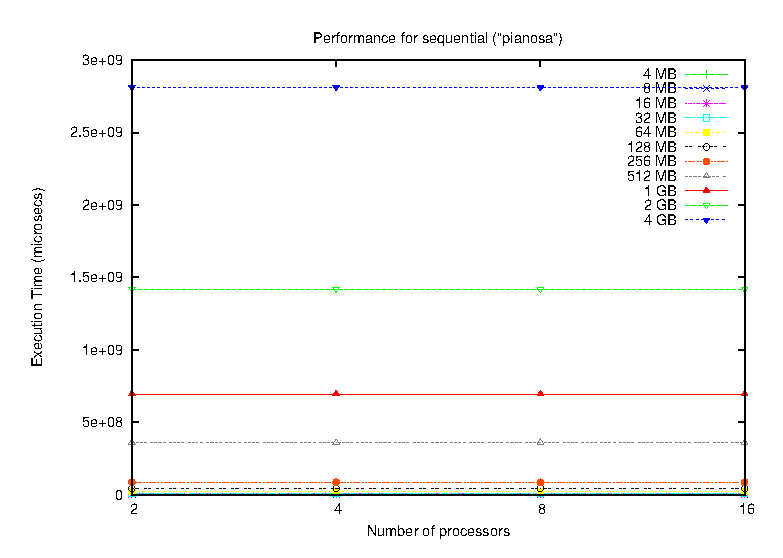
\includegraphics[scale=0.6]{plots/test_01_pianosa/NxTxM/sequential_pianosa_NxTxM}
	\end{center}
  	\caption{\textit{Pianosa}. Completion Time for the Sequentialsort.}
  	\label{sequential-pianosa}
\end{figure}

\begin{figure}[h]
	\centering
	\subfloat[Quicksort.]{\label{NxTxM-sequential}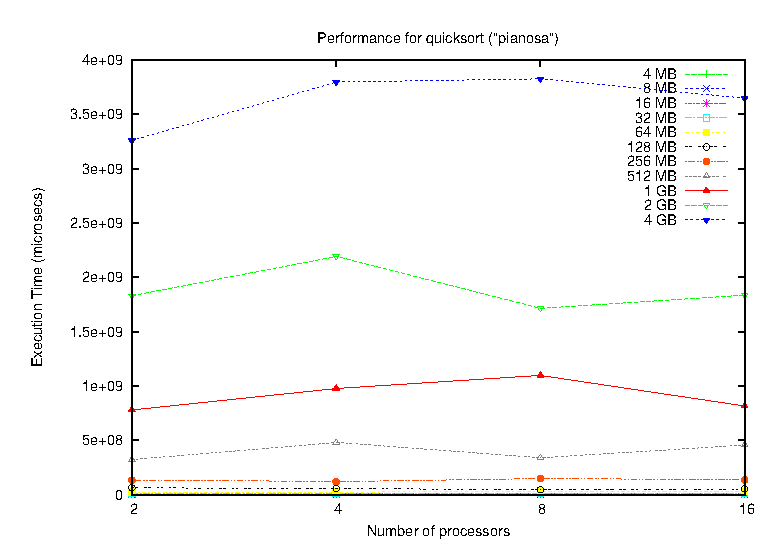
\includegraphics[width=0.4\textwidth]{plots/test_01_pianosa/NxTxM/quicksort_pianosa_NxTxM}} 
	\hspace*{20pt}	
  	\subfloat[Bitonicsort.]{\label{NxTxM-bitonicsort}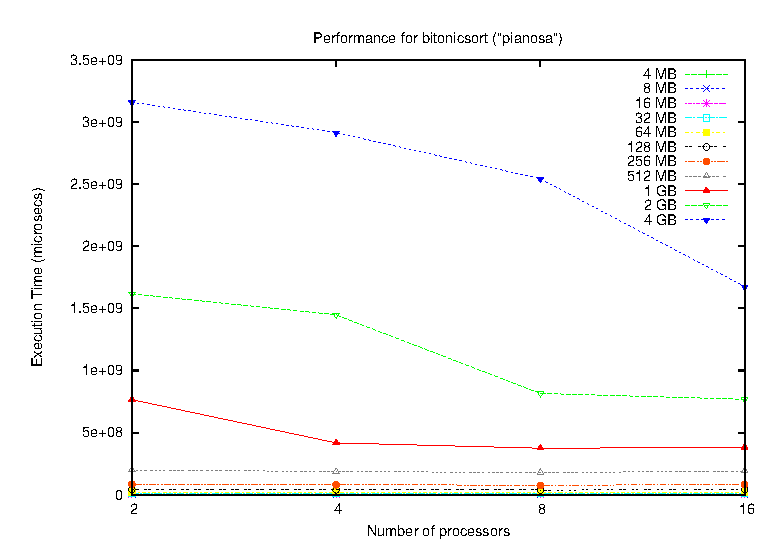
\includegraphics[width=0.4\textwidth]{plots/test_01_pianosa/NxTxM/bitonicsort_pianosa_NxTxM}} 
	
	\centering
	\subfloat[Bucketsort.]{\label{NxTxM-bucketsort}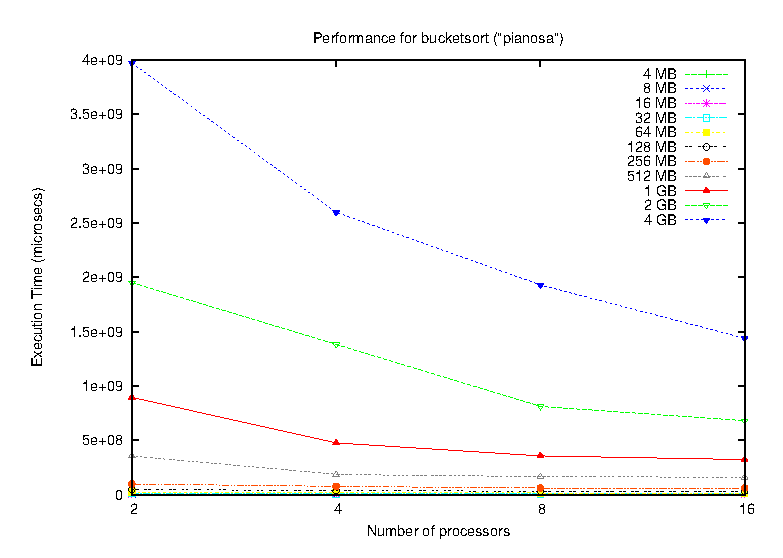
\includegraphics[width=0.4\textwidth]{plots/test_01_pianosa/NxTxM/bucketsort_pianosa_NxTxM}} 
  	\hspace*{20pt}
  	\subfloat[Samplesort.]{\label{NxTxM-samplesort}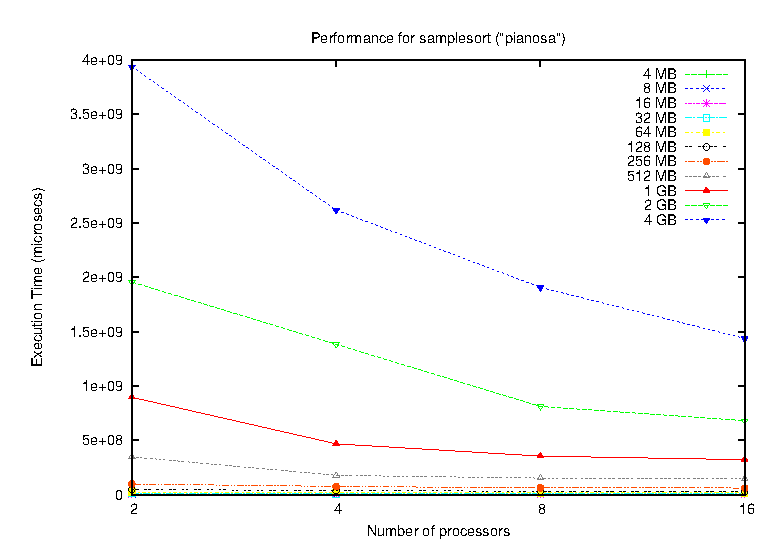
\includegraphics[width=0.4\textwidth]{plots/test_01_pianosa/NxTxM/samplesort_pianosa_NxTxM}} 
	
	\centering
  	\subfloat[Mergesort.]{\label{NxTxM-mergesort}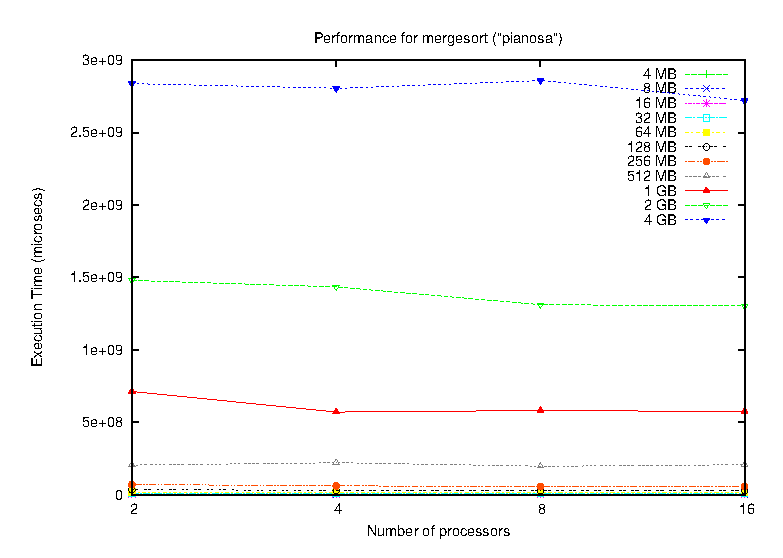
\includegraphics[width=0.4\textwidth]{plots/test_01_pianosa/NxTxM/mergesort_pianosa_NxTxM}}   
  	\hspace*{20pt}  
  	\subfloat[4-Way Mergesort.]{\label{NxTxM-kmerge}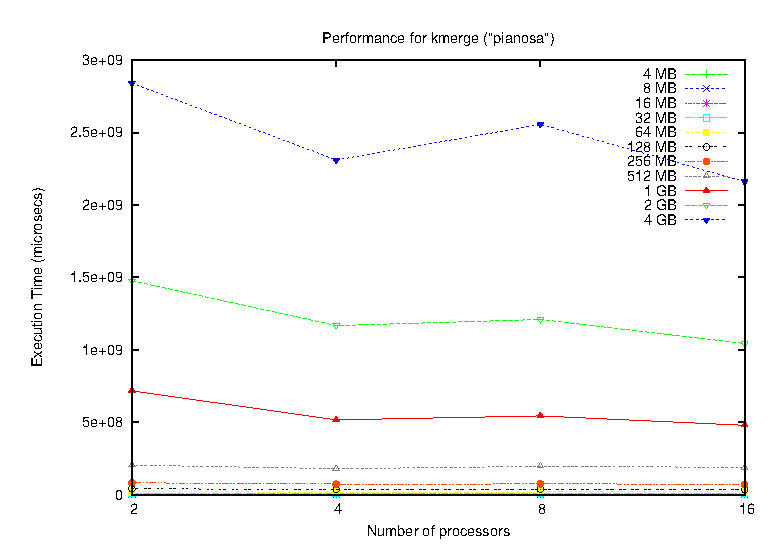
\includegraphics[width=0.4\textwidth]{plots/test_01_pianosa/NxTxM/kmerge_pianosa_NxTxM}} 
	
	\centering
  	\subfloat[Load-Balanced Mergesort.]{\label{NxTxM-lbmergesort}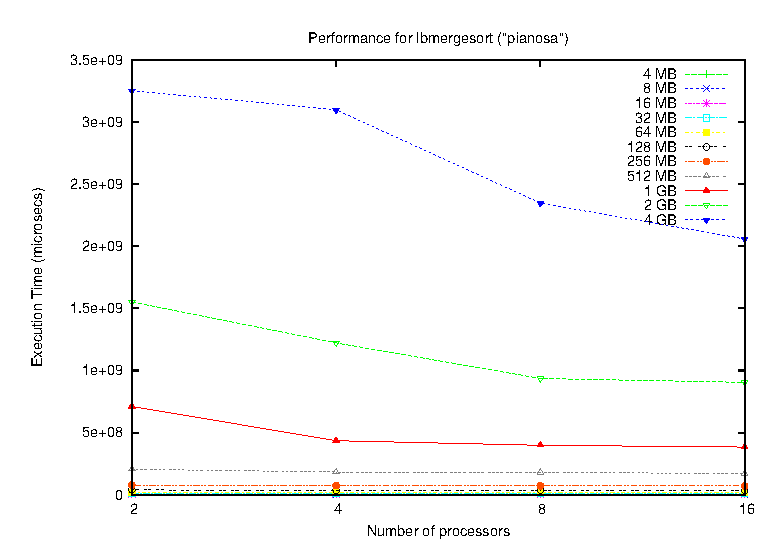
\includegraphics[width=0.4\textwidth]{plots/test_01_pianosa/NxTxM/lbmergesort_pianosa_NxTxM}} 
  	\hspace*{20pt}  
  	\subfloat[Load-Balanced Multi-Way Mergesort.]{\label{NxTxM-lbkmergesort}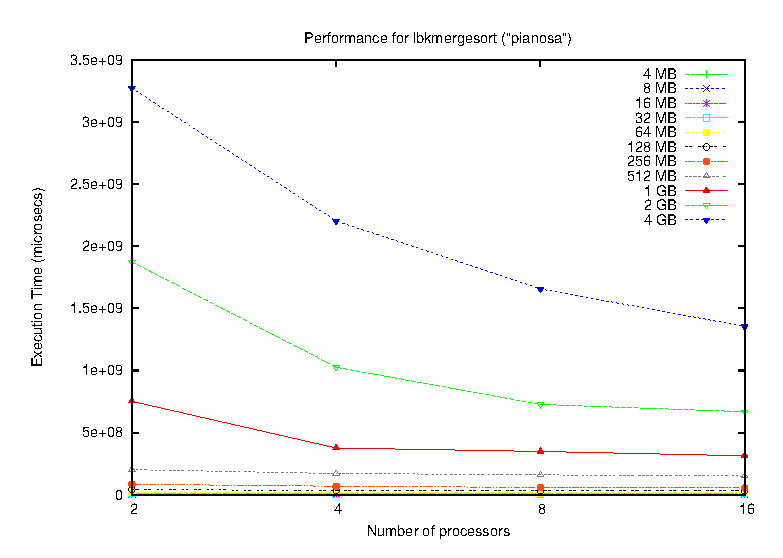
\includegraphics[width=0.4\textwidth]{plots/test_01_pianosa/NxTxM/lbkmergesort_pianosa_NxTxM}} 	
  	
	\caption{\textit{Pianosa}. Time Completion of Sorting Algorithms by varying the parallelism degree. Each shape on a graphic represents the Time Completion of a certain Sorting Algorithm for a data set of specific size.}
	\label{NxTxM}
\end{figure}
 
\begin{figure}[!ht]
	\centering
	\subfloat[Quicksort.]{\label{MxTxN-sequential}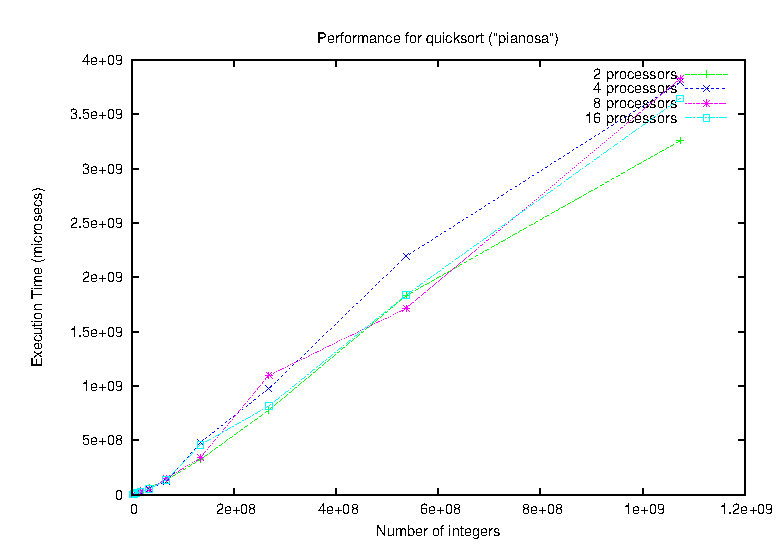
\includegraphics[width=0.4\textwidth]{plots/test_01_pianosa/MxTxN/quicksort_pianosa_MxTxN}} 
	\hspace*{20pt}	
  	\subfloat[Bitonicsort.]{\label{MxTxN-bitonicsort}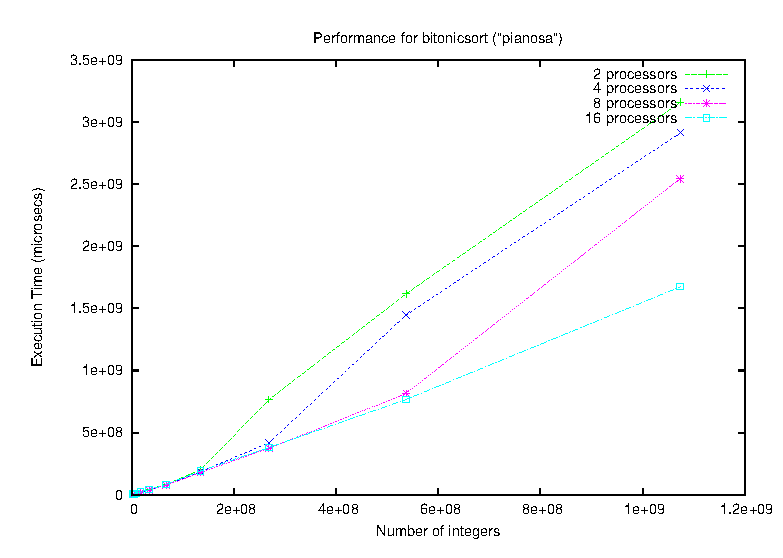
\includegraphics[width=0.4\textwidth]{plots/test_01_pianosa/MxTxN/bitonicsort_pianosa_MxTxN}} 
  		
	\centering
	\subfloat[Bucketsort.]{\label{MxTxN-bucketsort}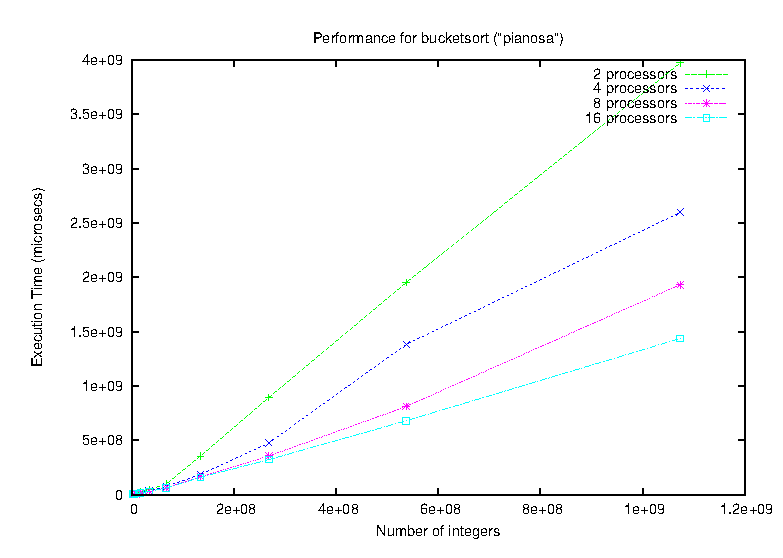
\includegraphics[width=0.4\textwidth]{plots/test_01_pianosa/MxTxN/bucketsort_pianosa_MxTxN}} 
  	\hspace*{20pt}
  	\subfloat[Samplesort.]{\label{MxTxN-samplesort}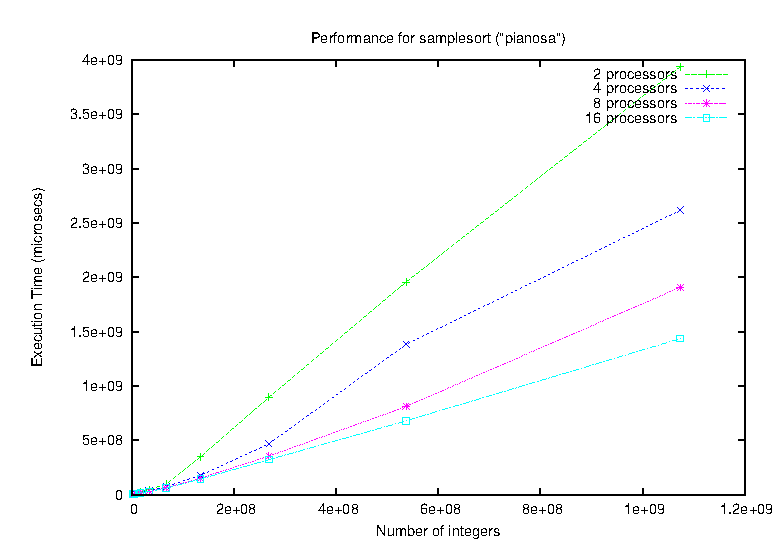
\includegraphics[width=0.4\textwidth]{plots/test_01_pianosa/MxTxN/samplesort_pianosa_MxTxN}} 
	
	\centering
  	\subfloat[Mergesort.]{\label{MxTxN-mergesort}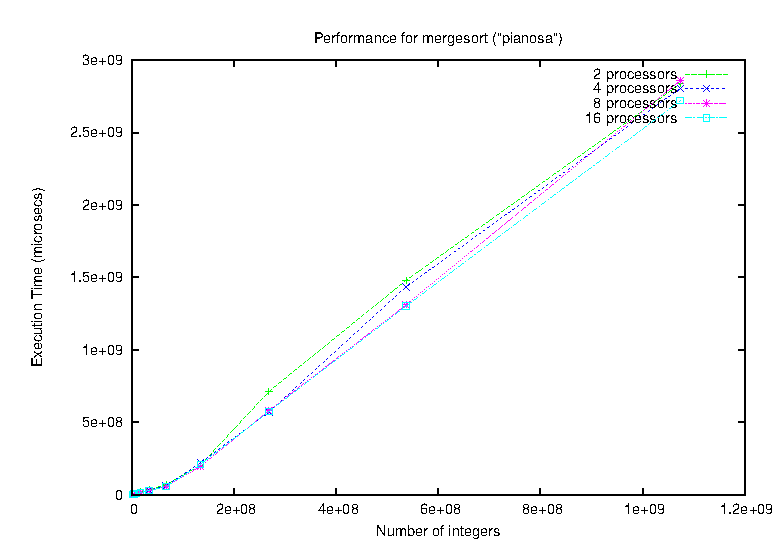
\includegraphics[width=0.4\textwidth]{plots/test_01_pianosa/MxTxN/mergesort_pianosa_MxTxN}}   
  	\hspace*{20pt}  
  	\subfloat[4-Way Mergesort.]{\label{MxTxN-kmerge}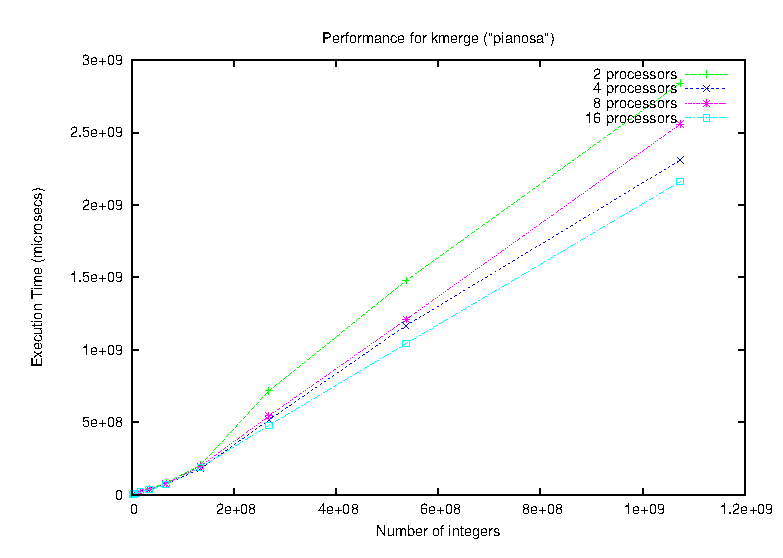
\includegraphics[width=0.4\textwidth]{plots/test_01_pianosa/MxTxN/kmerge_pianosa_MxTxN}} 
	
	\centering
  	\subfloat[Load-Balanced Mergesort.]{\label{MxTxN-lbmergesort}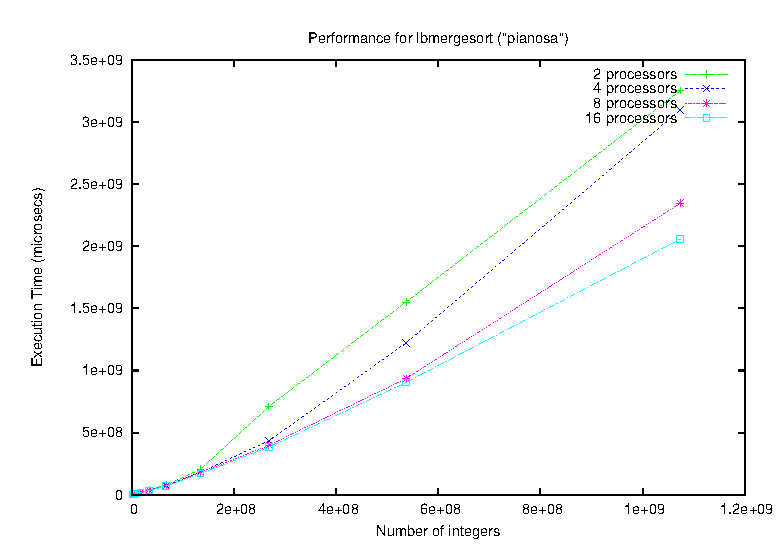
\includegraphics[width=0.4\textwidth]{plots/test_01_pianosa/MxTxN/lbmergesort_pianosa_MxTxN}} 
  	\hspace*{20pt}  
  	\subfloat[Load-Balanced Multi-Way Mergesort.]{\label{MxTxN-lbkmergesort}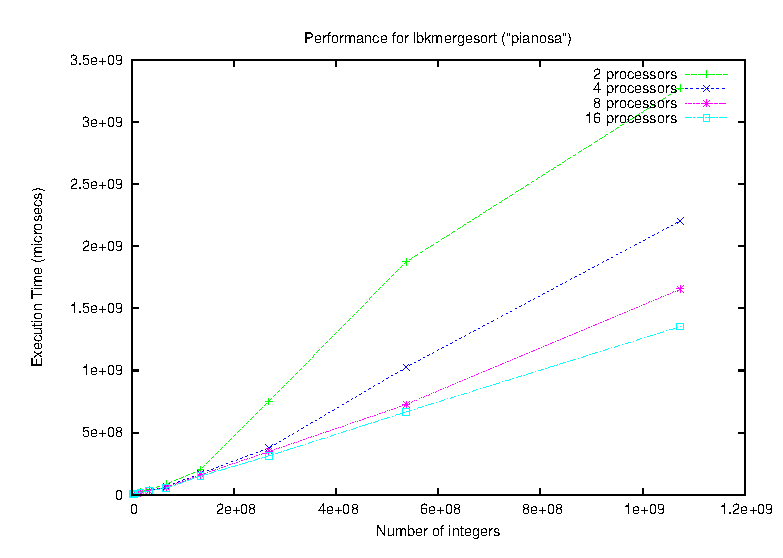
\includegraphics[width=0.4\textwidth]{plots/test_01_pianosa/MxTxN/lbkmergesort_pianosa_MxTxN}} 
  	
	\caption{\textit{Pianosa}. Time Completion of Sorting Algorithms for increasing sizes of the data set. }
	\label{MxTxN}
\end{figure} 
  
\paragraph{Comparison between Sorting Algorithms}
In the previous section we have analyzed the scalability of singles Sorting Algorithms for different sizes of the data set. Now, we focus on determining the best Sorting Algorithm, in terms of Time Completion, for different sizes of the data set. First of all, recall that whether a data set fits the primary memory, a call to \textit{Sequentialsort} is simply a call to the standard \textit{ANSI qsort} (see chapter~\ref{sort-fram}). Therefore, in case of \textbf{small} data sets, the \textit{Sequentialsort} is the best algorithm we can use. Indeed, as we have already anticipated, in these cases the overhead of the parallelization is greater than the time that we would spend in a sequential, optimized computation, like the one of \textit{qsort}. On the other hand, things are obvioulsy different for larger data sets. Figures~\ref{NxTxA-large} and~\ref{NxTxA-huge} can be used to derive which algorithms exhibit the best Time Completions respectively for large and huge data sets. First, we consider the case of \textbf{large} data sets. 
Aside the \textit{Quicksort}, which suffers the unbalancing of the load among processes (see Appendix~\ref{appendix} for more details), most of the Sorting Algorithms outperform \textit{Sequentialsort}, at least when the size of the data set is greater than 4M integers. At least up to parallelism degree 16, the best algorithm is \textit{Mergesort}: in the best case, it is able to lower the Time Completion of \textit{qsort} of roughly 25$\%$ (see Figure~\ref{NxTxA-32M}). Now, we move to \textit{huge} data sets. It has been a great pleasure to see that the \textit{Load-Balanced Multi-Way Mergesort} (the Sorting Algorithm we designed and implemented by taking cue from \textit{Load-Balanced Mergesort}) is the algorithm that shows \textit{always} the best Time Completion (see also Figures~\ref{MxTxA-n4},~\ref{MxTxA-n8} and~\ref{MxTxA-n16}). Unfortunately, the lack of further machines to increase the parallelism degree at least up to 32 prevents the possibility of claiming deeper conclusions on these aspects. 


\begin{figure}[!ht]
	\centering
	\subfloat[Data set of 1M integers.]{\label{NxTxA-1M}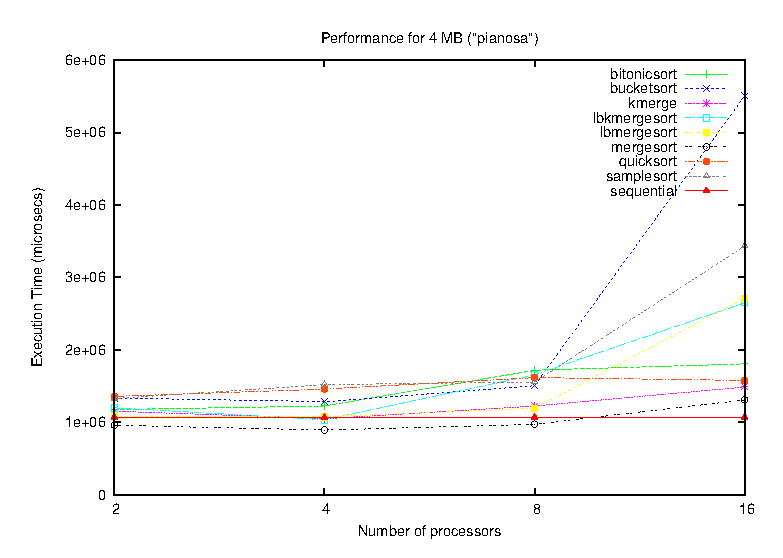
\includegraphics[width=0.4\textwidth]{plots/test_01_pianosa/NxTxA/M1048576_pianosa_NxTxA}} 
	\hspace*{20pt}	
  	\subfloat[Data set of 2M integers.]{\label{NxTxA-2M}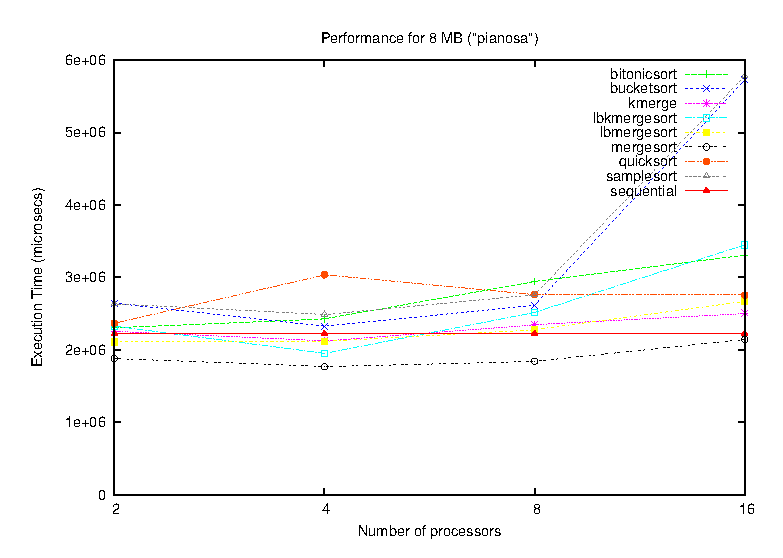
\includegraphics[width=0.4\textwidth]{plots/test_01_pianosa/NxTxA/M2097152_pianosa_NxTxA}} 
  		
	\centering
	\subfloat[Data set of 4M integers.]{\label{NxTxA-4M}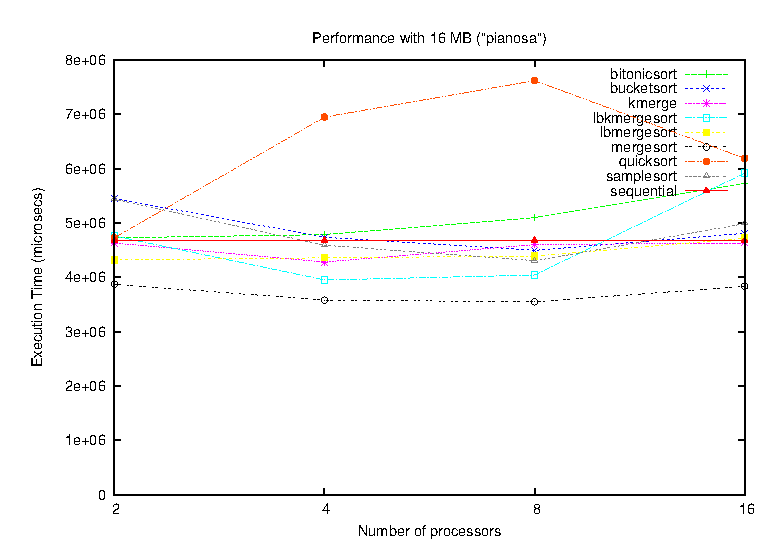
\includegraphics[width=0.4\textwidth]{plots/test_01_pianosa/NxTxA/M4194304_pianosa_NxTxA}} 
  	\hspace*{20pt}
  	\subfloat[Data set of 8M integers.]{\label{NxTxA-8M}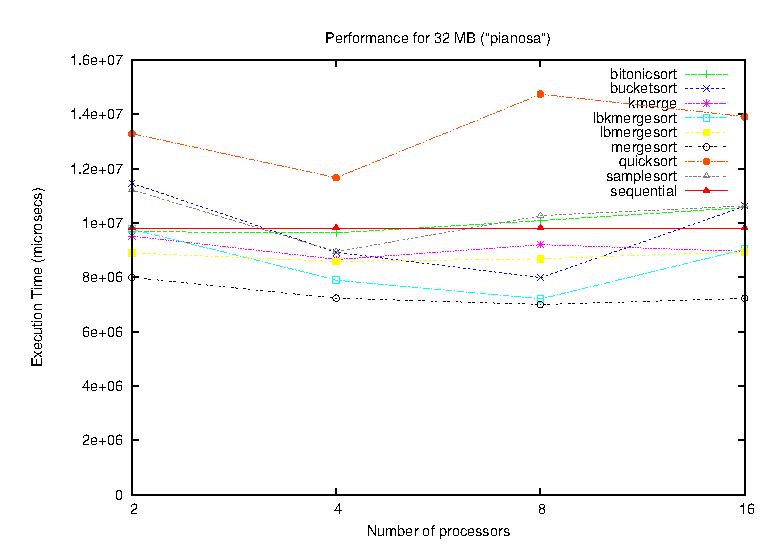
\includegraphics[width=0.4\textwidth]{plots/test_01_pianosa/NxTxA/M8388608_pianosa_NxTxA}} 
	
	\centering
  	\subfloat[Data set of 16M integers.]{\label{NxTxA-16M}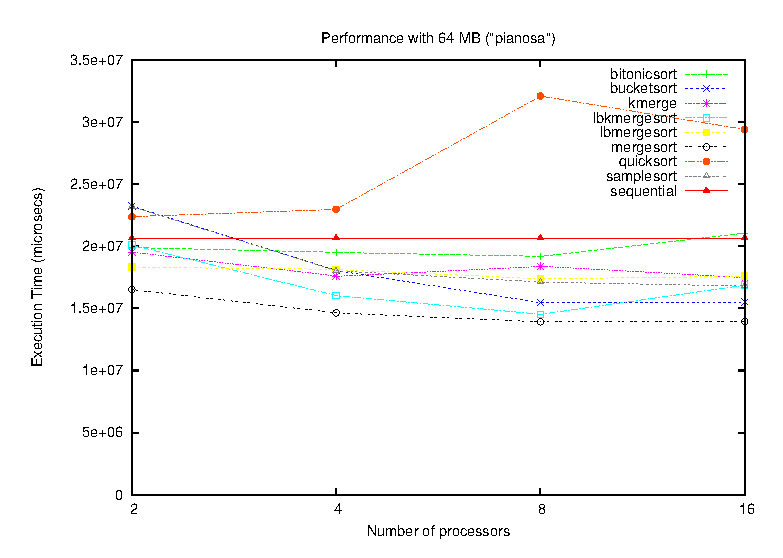
\includegraphics[width=0.4\textwidth]{plots/test_01_pianosa/NxTxA/M16777216_pianosa_NxTxA}}   
  	\hspace*{20pt}  
  	\subfloat[Data set of 32M integers.]{\label{NxTxA-32M}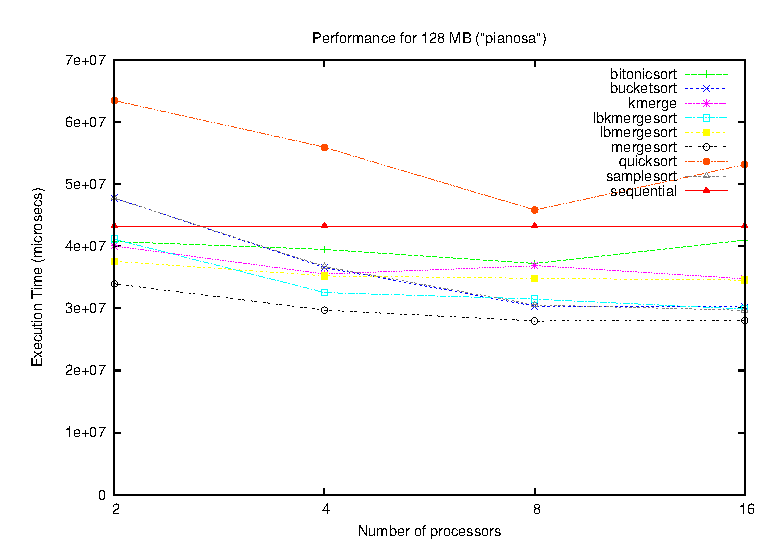
\includegraphics[width=0.4\textwidth]{plots/test_01_pianosa/NxTxA/M33554432_pianosa_NxTxA}} 
  	
	\caption{\textit{Pianosa}. Time Completion for sorting \textit{small} data sets. Each graphic represents a data set of fixed size, while each shape on a graphic shows the Time Completion of a certain Sorting Algorithm for that data set.}
	\label{NxTxA-small}
\end{figure} 

\begin{figure}[!ht]
	\centering
	\subfloat[Data set of 64M integers.]{\label{NxTxA-64M}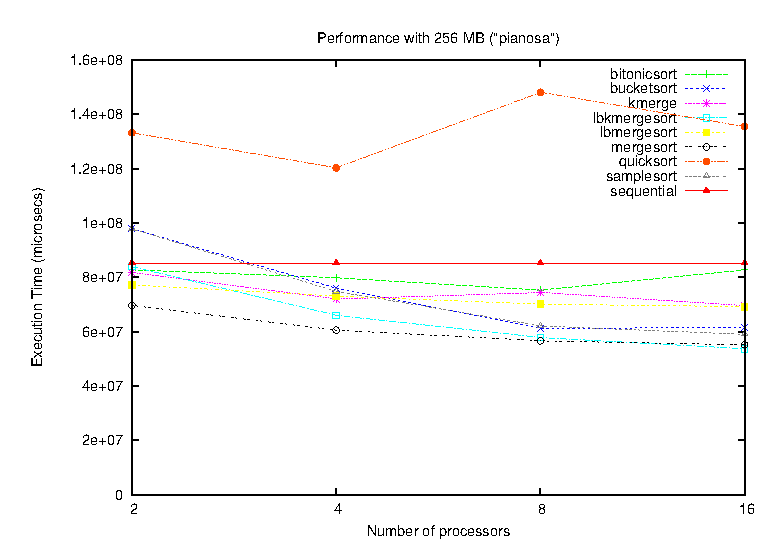
\includegraphics[width=0.5\textwidth]{plots/test_01_pianosa/NxTxA/M67108864_pianosa_NxTxA}} 
	
	\centering
  	\subfloat[Data set of 128M integers.]{\label{NxTxA-128M}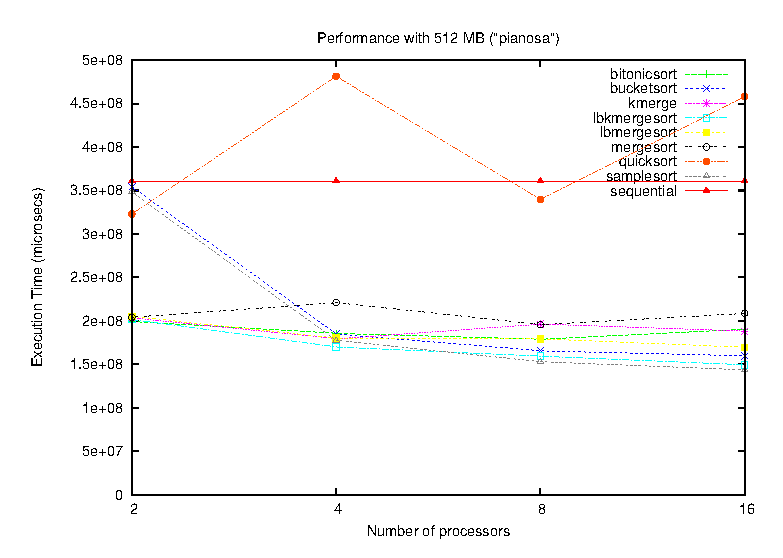
\includegraphics[width=0.5\textwidth]{plots/test_01_pianosa/NxTxA/M134217728_pianosa_NxTxA}} 
  		
	\centering
	\subfloat[Data set of 256M integers.]{\label{NxTxA-256M}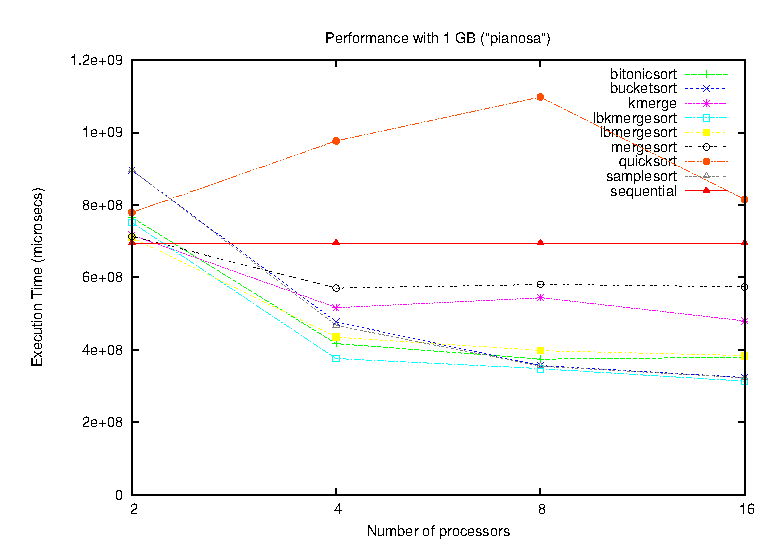
\includegraphics[width=0.5\textwidth]{plots/test_01_pianosa/NxTxA/M268435456_pianosa_NxTxA}} 
  	
  	\caption{\textit{Pianosa}. Time Completion for sorting \textit{large} data sets. Each graphic represents a data set of fixed size, while each shape on a graphic shows the Time Completion of a certain Sorting Algorithm for that data set.}
	\label{NxTxA-large}
\end{figure}

\begin{figure}[!ht]  	
  	\centering
  	\subfloat[Data set of 512M integers.]{\label{NxTxA-512M}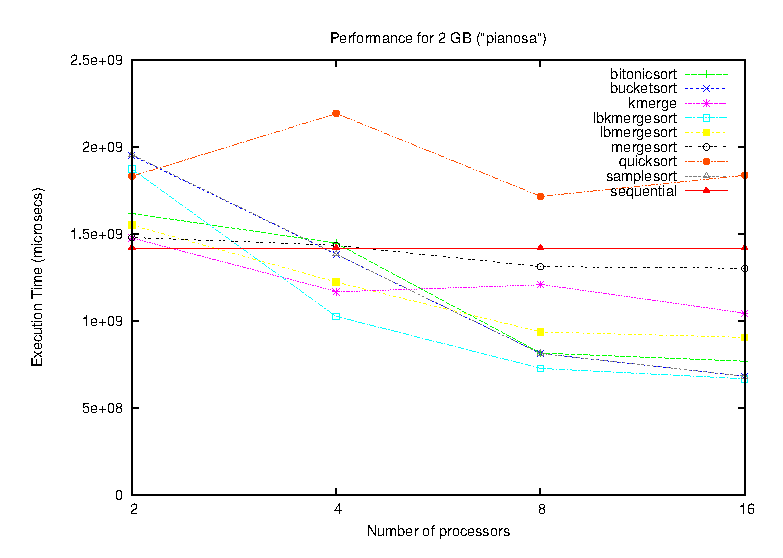
\includegraphics[width=0.6\textwidth]{plots/test_01_pianosa/NxTxA/M536870912_pianosa_NxTxA}} 
	
	\centering
  	\subfloat[Data set of 1G integers.]{\label{NxTxA-1G}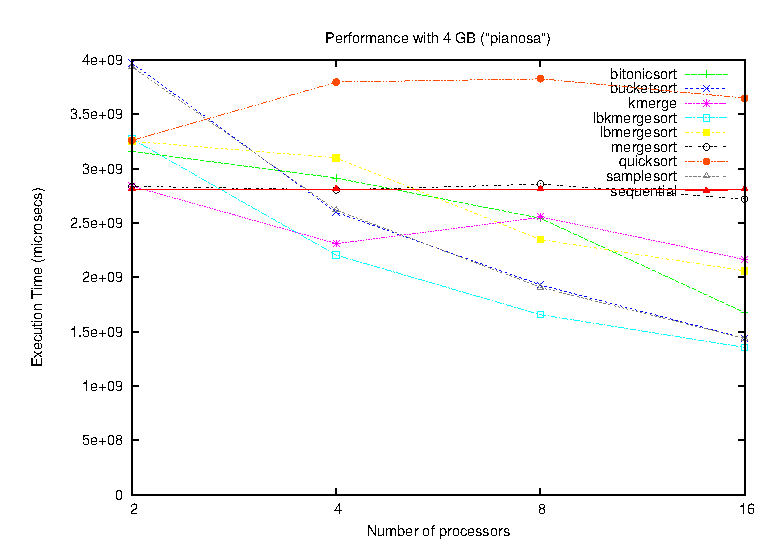
\includegraphics[width=0.6\textwidth]{plots/test_01_pianosa/NxTxA/M1073741824_pianosa_NxTxA}}    
  	
	\caption{\textit{Pianosa}. Time Completion for sorting \textit{huge} data sets. Each graphic represents a data set of fixed size, while each shape on a graphic shows the Time Completion of a certain Sorting Algorithm for that data set.}
	\label{NxTxA-huge}
\end{figure} 

\begin{figure}[!ht]
	\centering
	\subfloat[Parallelism degree 2.]{\label{MxTxA-n2}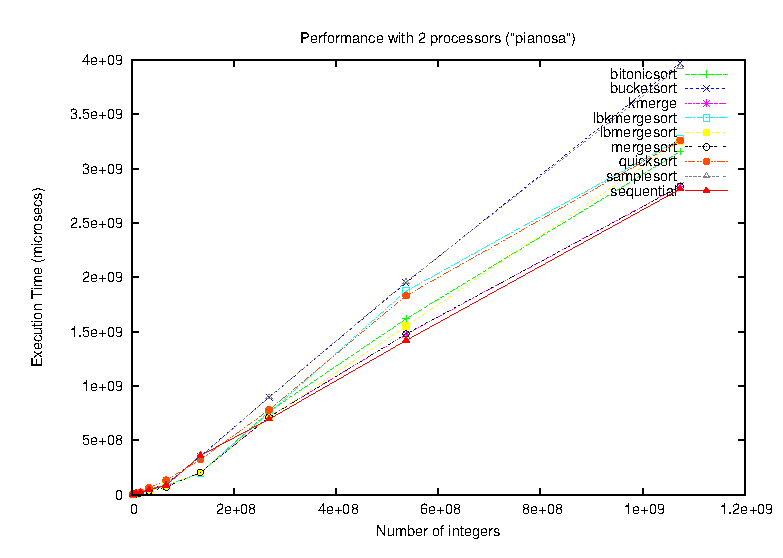
\includegraphics[width=0.4\textwidth]{plots/test_01_pianosa/MxTxA/n2_pianosa_MxTxA}} 
	\hspace*{20pt}	
  	\subfloat[Parallelism degree 4.]{\label{MxTxA-n4}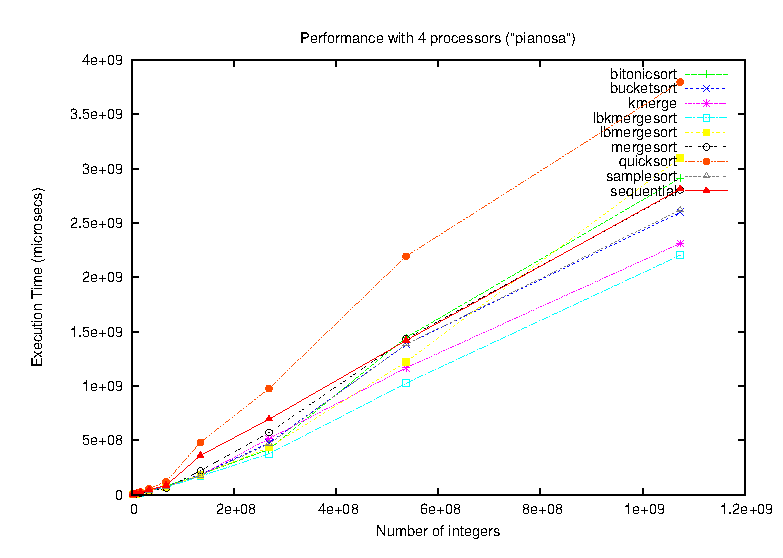
\includegraphics[width=0.4\textwidth]{plots/test_01_pianosa/MxTxA/n4_pianosa_MxTxA}} 
  		
	\centering
	\subfloat[Parallelism degree 8.]{\label{MxTxA-n8}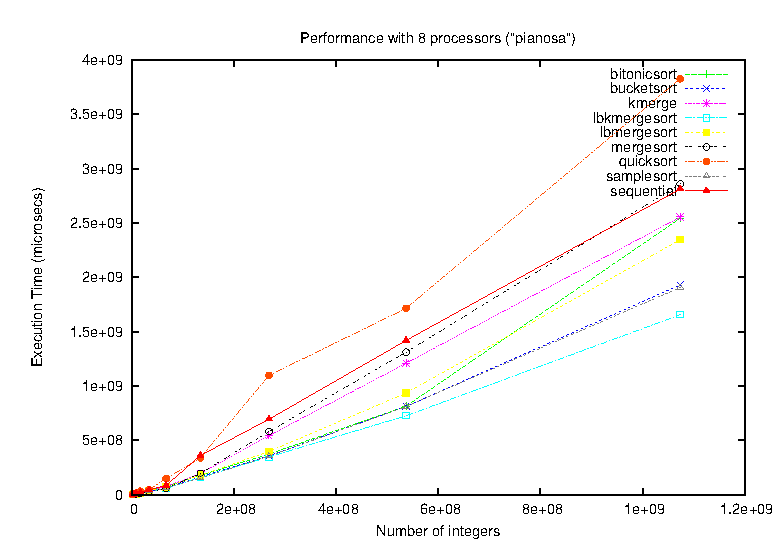
\includegraphics[width=0.4\textwidth]{plots/test_01_pianosa/MxTxA/n8_pianosa_MxTxA}} 
  	\hspace*{20pt}
  	\subfloat[Parallelism degree 16.]{\label{MxTxA-n16}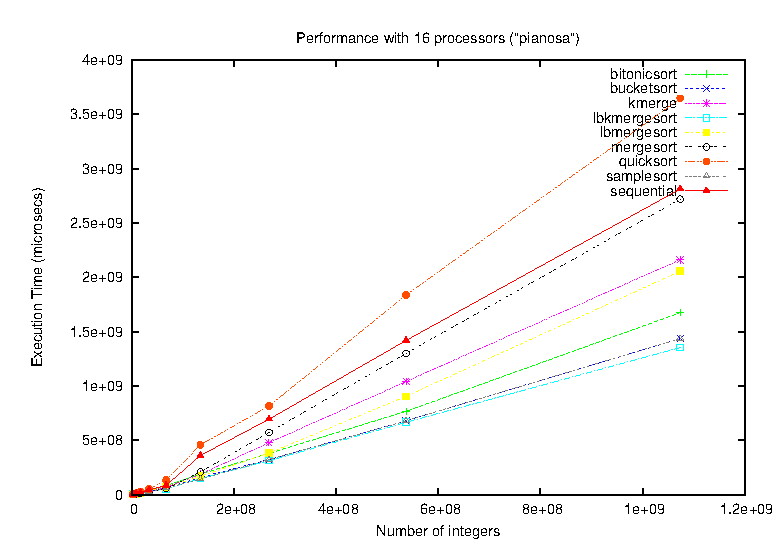
\includegraphics[width=0.4\textwidth]{plots/test_01_pianosa/MxTxA/n16_pianosa_MxTxA}} 
  	
	\caption{\textit{Pianosa}. Time Completion for sorting data sets with fixed parallelism degree.}
	\label{MxTxA}
\end{figure} 

\clearpage
\subsubsection{Intel Xeon X5670}
In this section we analyze the behavior of Sorting Algorithms on a Chip MultiProcessor (CMP), namely a Symmetric MultiProcessor (SMP) on chip. The CMP in question is a generic node of the cluster $PCM$, the Intel Xeon X5670 described in~\ref{PCM}. We will be able to test our algorithms for parallelism degrees up to 8. We expect that performance results on this architecture will be significantly different from the ones obtained on Pianosa, in particular from a \textit{qualitative} point of view. Indeed, there are at least two key factors that can drastically impact on the performance: first, the huge amount of primary memory will diminish the overhead due to I/Os; second, the communications now take place in shared memory thus they are less expensive.


\begin{figure}[t]
    \begin{center}
        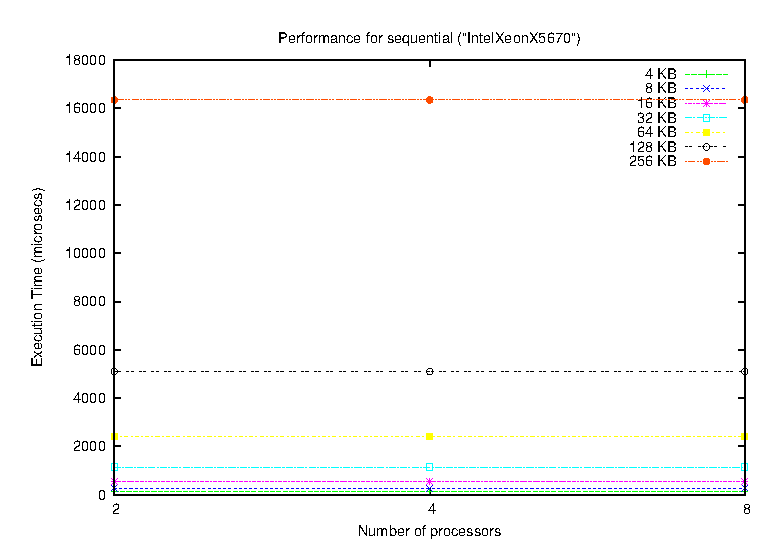
\includegraphics[scale=0.6]{plots/test_01_IntelXeonX5670/NxTxM/sequential_IntelXeonX5670_NxTxM_small}
    \end{center}
    
    \begin{center}
        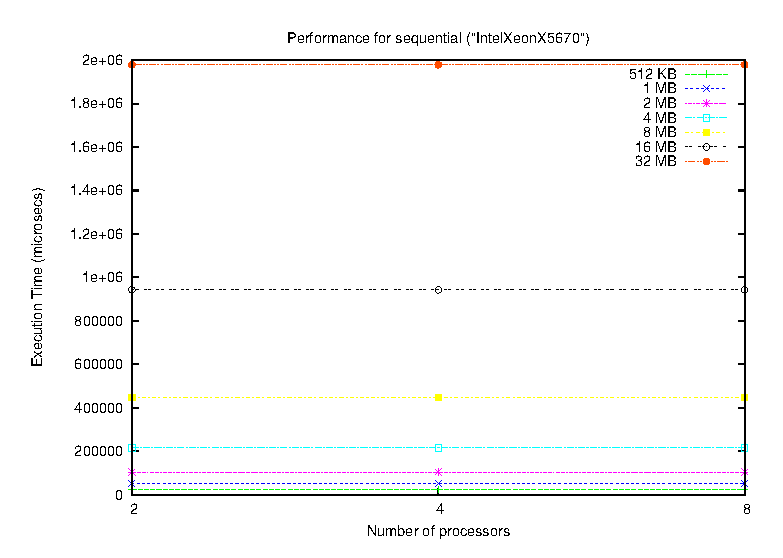
\includegraphics[scale=0.6]{plots/test_01_IntelXeonX5670/NxTxM/sequential_IntelXeonX5670_NxTxM_large}
    \end{center}
    
    \begin{center}
        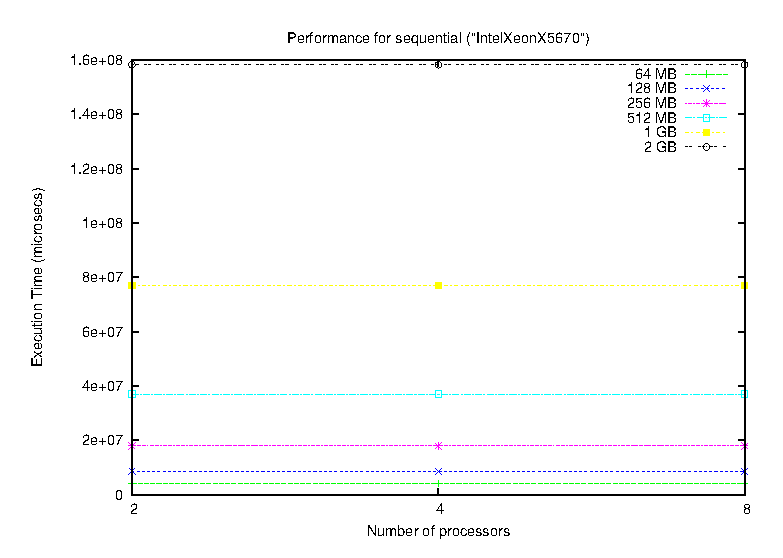
\includegraphics[scale=0.6]{plots/test_01_IntelXeonX5670/NxTxM/sequential_IntelXeonX5670_NxTxM_huge}
    \end{center}
    \caption{\textit{IntelXeonX5670}. Completion Time for the Sequentialsort.}
    \label{sequential-IntelXeonX5670}
\end{figure}

\paragraph{Scalability of Sorting Algorithms} Figure~\ref{IntelXeonX5670-NxTxM} and~\ref{IntelXeonX5670-MxTxN} show the time completion of Sorting Algorithms for data sets up to 2 GB. Exactly as on $Pianosa$, due to the fine grain computation, there is not any Sorting Algorithm that shows a good scalability for \textbf{small} data sets. On the other hand, the previous considerations on the primary memory size and the cost of communications justify intuitively why, for \textbf{large} data sets, most Sorting Algorithms scale better than on $Pianosa$ (even if still far away from the ideality). Figure~\ref{IntelXeonX5670-NxTxM} shows that increasing the parallelism degree from 2 to 4, a lot of Sorting Algorithms scale really close to the ideality, while from 4 to 8 there is still a gain, but in general lower. Exactly as on $Pianosa$, \textit{Bucketsort}, \textit{Samplesort} and \textit{Load-Balanced Multi-Way Mergesort} exhibit the best performance in terms of both scalability and time completion. \textit{Mergesort} (Figure~\ref{IntelXeonX5670-NxTxM-mergesort}) was bad on $Pianosa$ because of both the communications overhead and the unbalanced workload, but now exhibit a great scalability up to parallelism degree 8; this is thanks also to the faster hardware which let the last sequential phase of merging to become less incisive on the overall time completion. Figure~\ref{IntelXeonX5670-NxTxM-quicksort} shows \textit{Quicksort}; this algorithm exhibit the worst performance for what concern both the scalability and the absolute Time Completion. This is likely due to the fact that the load gets unbalanced between the processes of the computation (see Appendix~\ref{appendix} for more details). Figure~\ref{IntelXeonX5670-NxTxM-kmerge} shows the bad performance of \textit{4-Way Mergesort}; this algorithm suffers the last phase of merging that, since it is made by a single process (see~\ref{kmerge}), becomes predominant with respect to the gain of the parallelization. 




%%%%%%%%%%%%%%%%%%%%%%%%%%%%%%%%%%%%%%%% Small data set %%%%%%%%%%%%%%%%%%%%%%%%%%%%%%%%%%%%%%%%%%%%%%%%%%%%%%
\begin{figure}[h]
    \centering
    \subfloat[Quicksort.]{\label{NxTxM_small-quicksort}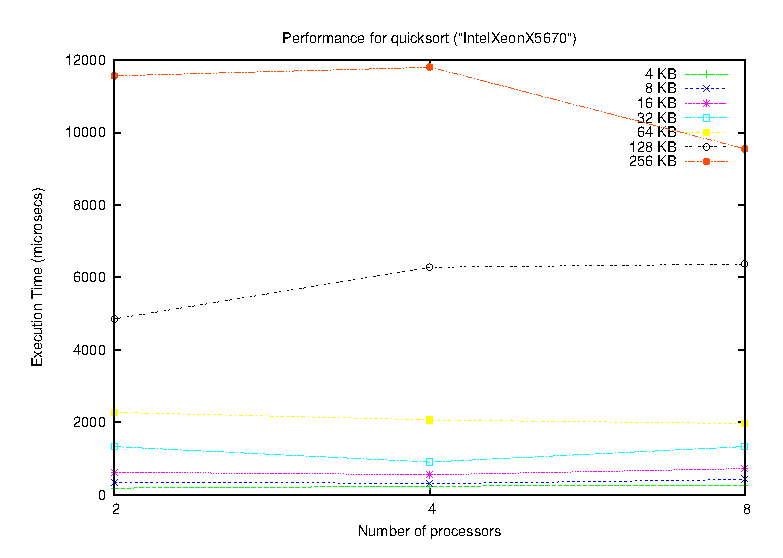
\includegraphics[width=0.4\textwidth]{plots/test_01_IntelXeonX5670/NxTxM/quicksort_IntelXeonX5670_NxTxM_small}} 
    \hspace*{20pt}  
    \subfloat[Bitonicsort.]{\label{NxTxM_small-bitonicsort}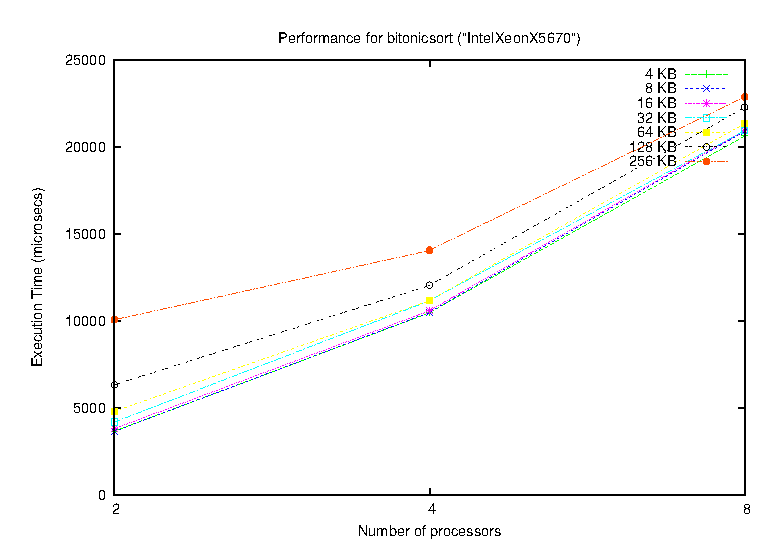
\includegraphics[width=0.4\textwidth]{plots/test_01_IntelXeonX5670/NxTxM/bitonicsort_IntelXeonX5670_NxTxM_small}} 
    
    \centering
    \subfloat[Bucketsort.]{\label{NxTxM_small-bucketsort}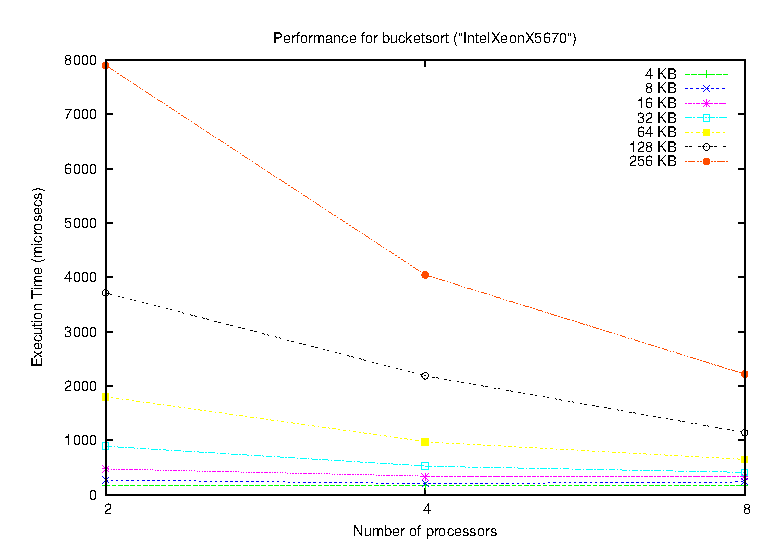
\includegraphics[width=0.4\textwidth]{plots/test_01_IntelXeonX5670/NxTxM/bucketsort_IntelXeonX5670_NxTxM_small}} 
    \hspace*{20pt}
    \subfloat[Samplesort.]{\label{NxTxM_small-samplesort}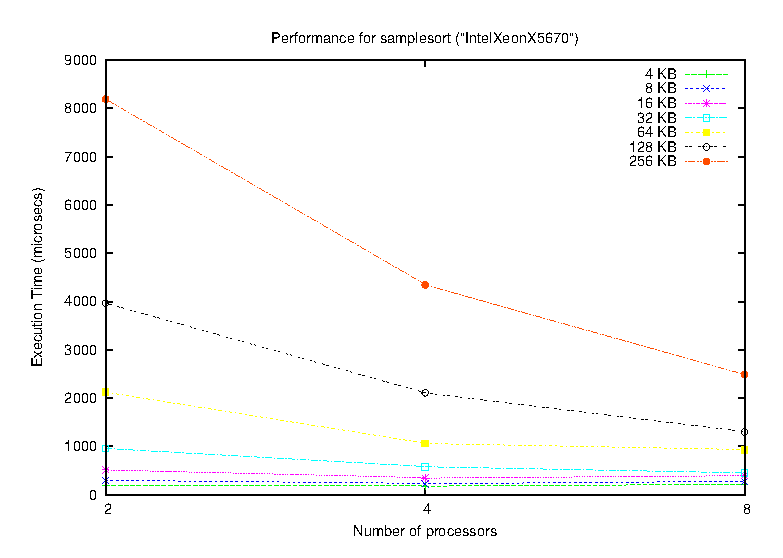
\includegraphics[width=0.4\textwidth]{plots/test_01_IntelXeonX5670/NxTxM/samplesort_IntelXeonX5670_NxTxM_small}} 
    
    \centering
    \subfloat[Mergesort.]{\label{NxTxM_small-mergesort}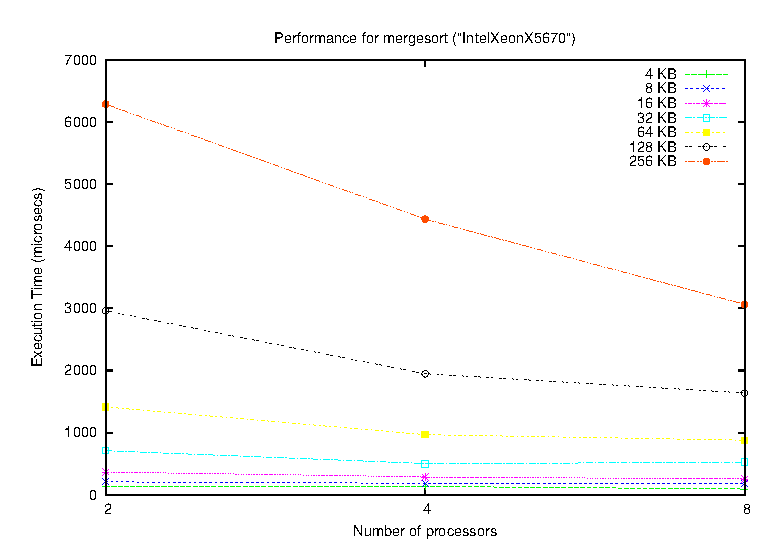
\includegraphics[width=0.4\textwidth]{plots/test_01_IntelXeonX5670/NxTxM/mergesort_IntelXeonX5670_NxTxM_small}}   
    \hspace*{20pt}  
    \subfloat[4-Way Mergesort.]{\label{NxTxM_small-kmerge}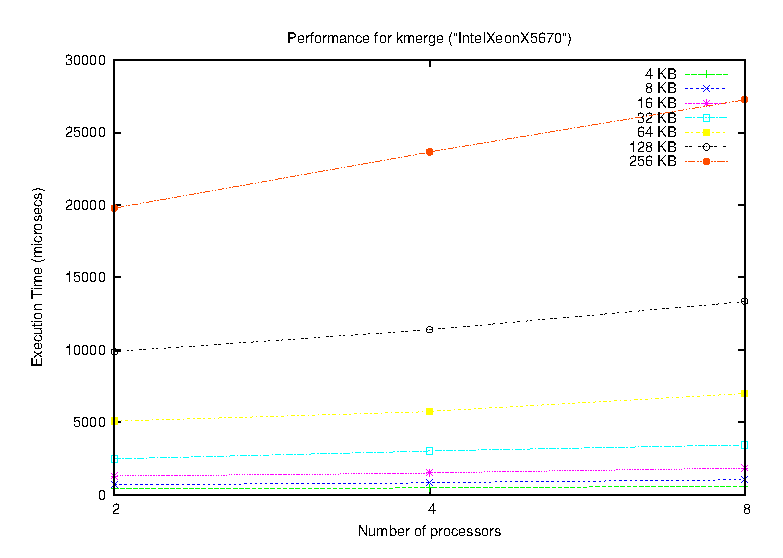
\includegraphics[width=0.4\textwidth]{plots/test_01_IntelXeonX5670/NxTxM/kmerge_IntelXeonX5670_NxTxM_small}} 
    
    \centering
    \subfloat[Load-Balanced Mergesort.]{\label{NxTxM_small-lbmergesort}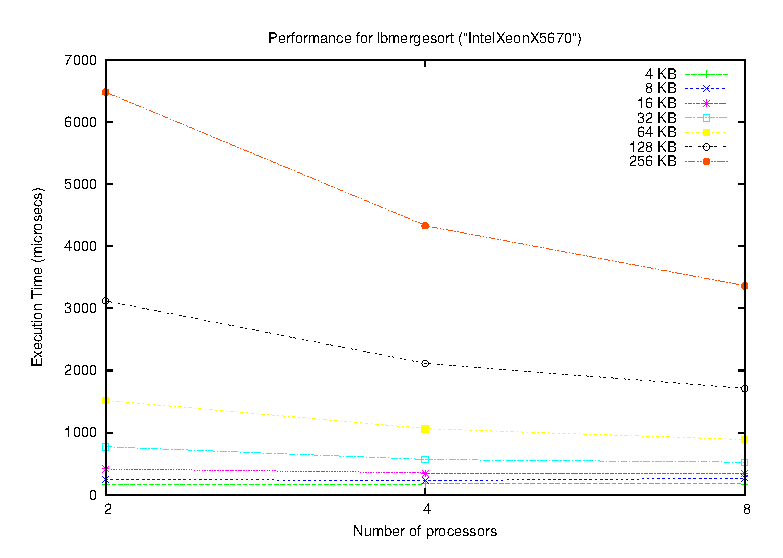
\includegraphics[width=0.4\textwidth]{plots/test_01_IntelXeonX5670/NxTxM/lbmergesort_IntelXeonX5670_NxTxM_small}} 
    \hspace*{20pt}  
    \subfloat[Load-Balanced Multi-Way Mergesort.]{\label{NxTxM_small-lbkmergesort}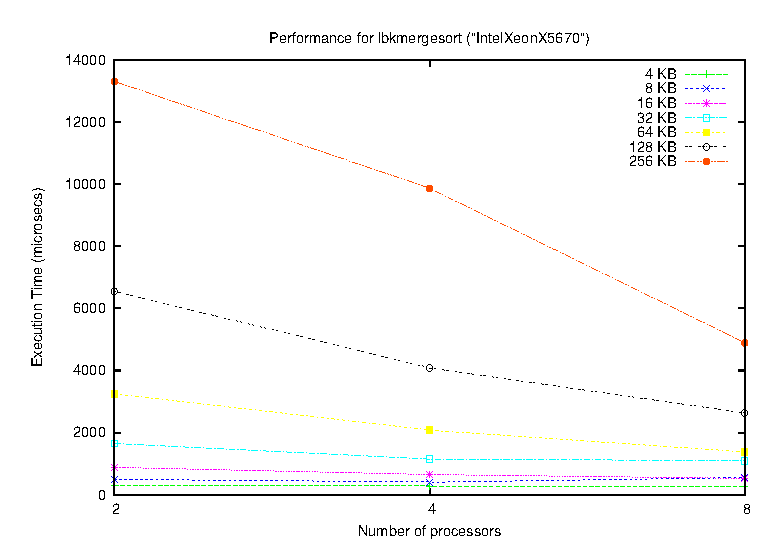
\includegraphics[width=0.4\textwidth]{plots/test_01_IntelXeonX5670/NxTxM/lbkmergesort_IntelXeonX5670_NxTxM_small}}  
    
\end{figure}



  
%%%%%%%%%%%%%%%%%%%%%%%%%%%%%%%%%%%%%%%% Large data set %%%%%%%%%%%%%%%%%%%%%%%%%%%%%%%%%%%%%%%%%%%%%%%%%%%%%%
\begin{figure}[h]	
	\ContinuedFloat
	
    \centering
    \subfloat[Quicksort.]{\label{NxTxM_large-quicksort}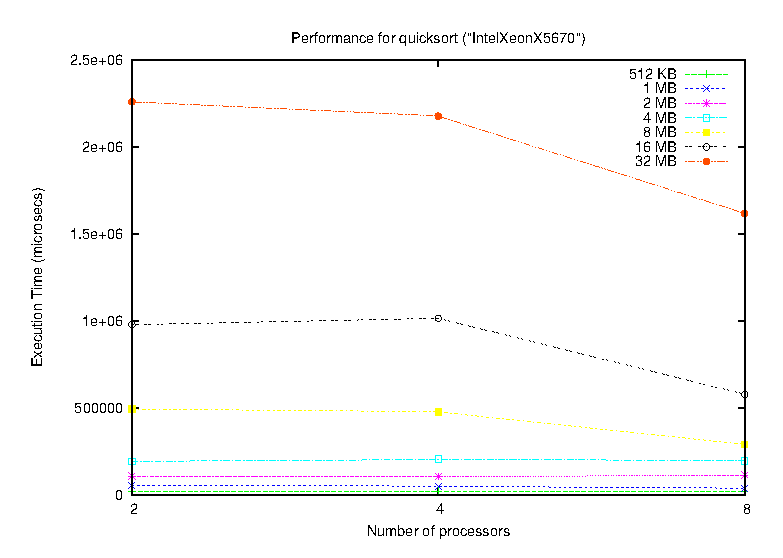
\includegraphics[width=0.4\textwidth]{plots/test_01_IntelXeonX5670/NxTxM/quicksort_IntelXeonX5670_NxTxM_large}} 
    \hspace*{20pt}  
    \subfloat[Bitonicsort.]{\label{NxTxM_large-bitonicsort}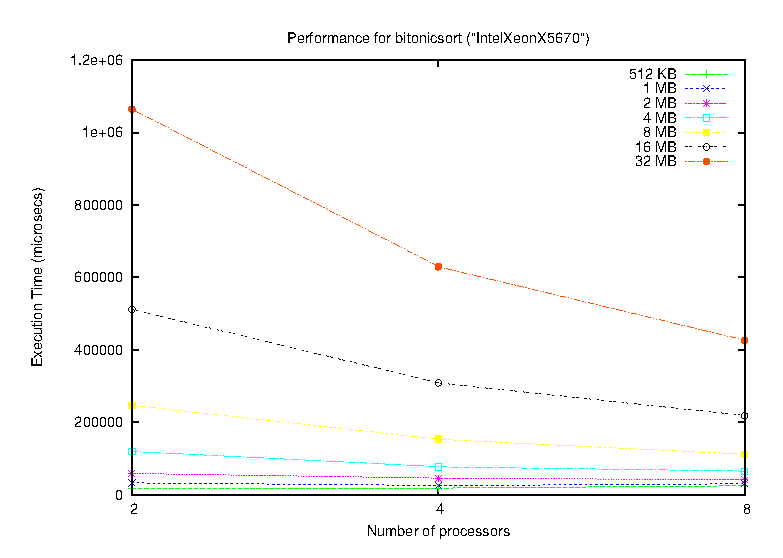
\includegraphics[width=0.4\textwidth]{plots/test_01_IntelXeonX5670/NxTxM/bitonicsort_IntelXeonX5670_NxTxM_large}} 
    
    \centering
    \subfloat[Bucketsort.]{\label{NxTxM_large-bucketsort}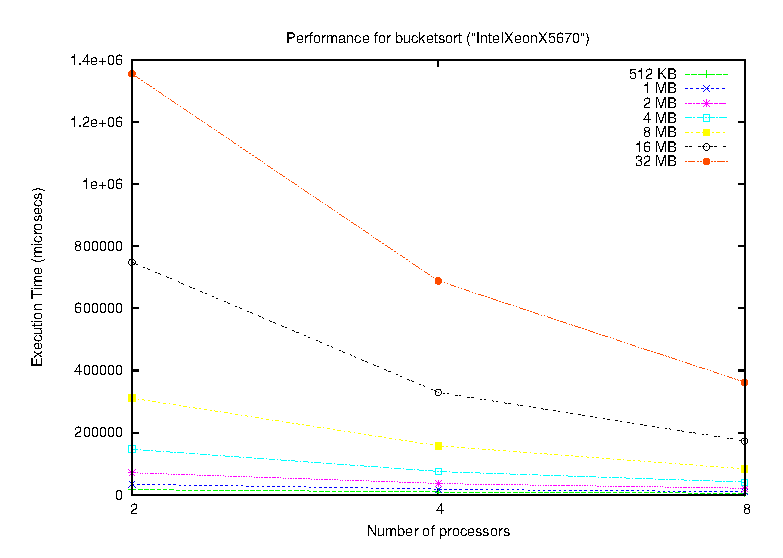
\includegraphics[width=0.4\textwidth]{plots/test_01_IntelXeonX5670/NxTxM/bucketsort_IntelXeonX5670_NxTxM_large}} 
    \hspace*{20pt}
    \subfloat[Samplesort.]{\label{NxTxM_large-samplesort}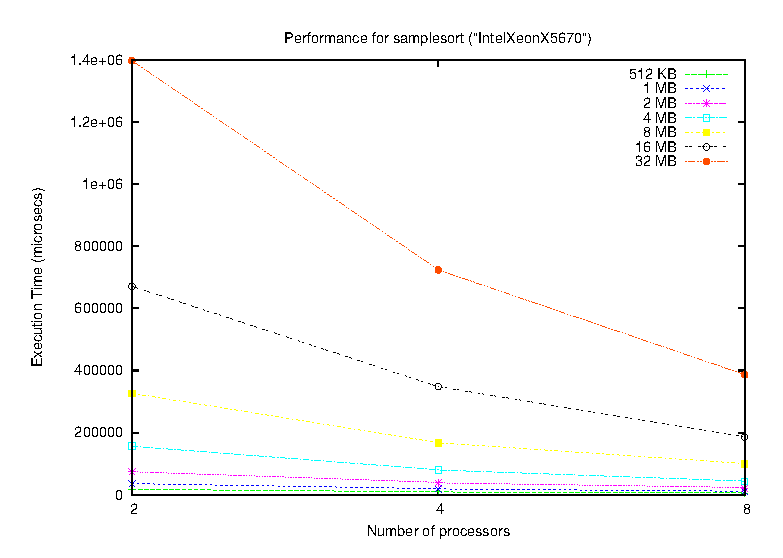
\includegraphics[width=0.4\textwidth]{plots/test_01_IntelXeonX5670/NxTxM/samplesort_IntelXeonX5670_NxTxM_large}} 
    
    \centering
    \subfloat[Mergesort.]{\label{NxTxM_large-mergesort}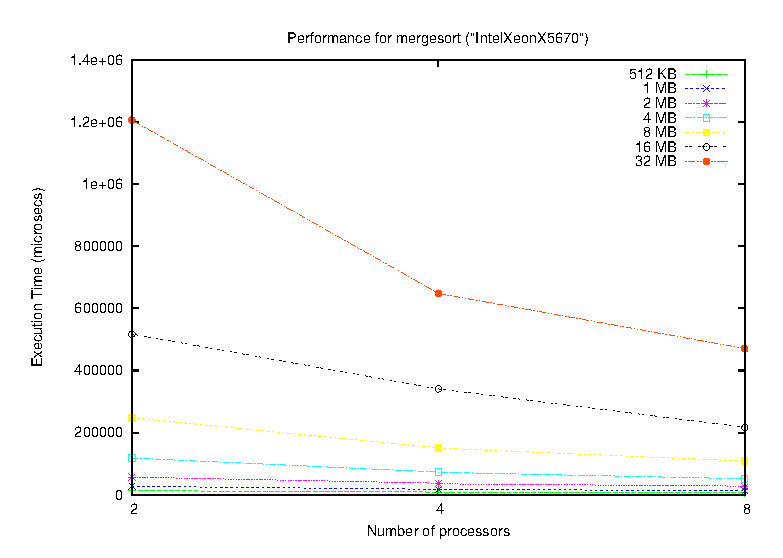
\includegraphics[width=0.4\textwidth]{plots/test_01_IntelXeonX5670/NxTxM/mergesort_IntelXeonX5670_NxTxM_large}}   
    \hspace*{20pt}  
    \subfloat[4-Way Mergesort.]{\label{NxTxM_large-kmerge}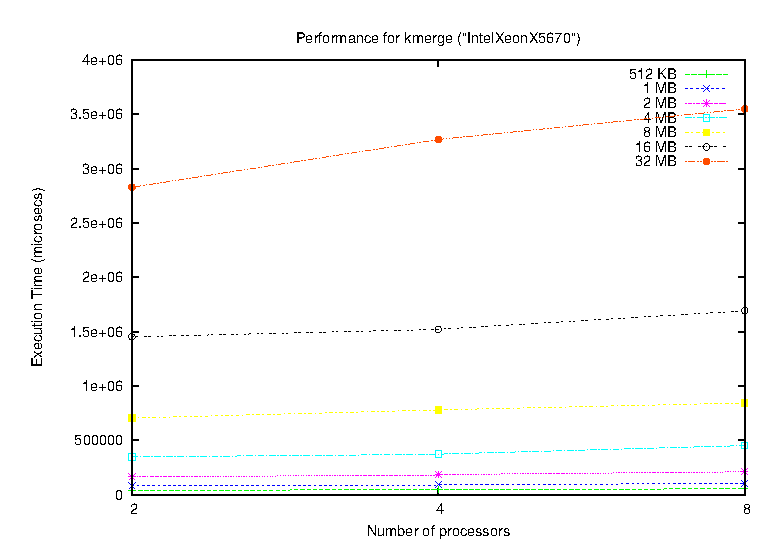
\includegraphics[width=0.4\textwidth]{plots/test_01_IntelXeonX5670/NxTxM/kmerge_IntelXeonX5670_NxTxM_large}} 
    
    \centering
    \subfloat[Load-Balanced Mergesort.]{\label{NxTxM_large-lbmergesort}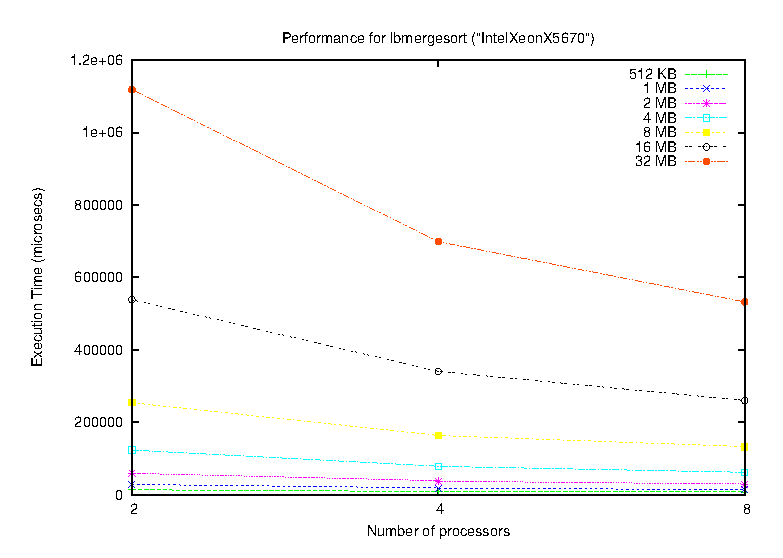
\includegraphics[width=0.4\textwidth]{plots/test_01_IntelXeonX5670/NxTxM/lbmergesort_IntelXeonX5670_NxTxM_large}} 
    \hspace*{20pt}  
    \subfloat[Load-Balanced Multi-Way Mergesort.]{\label{NxTxM_large-lbkmergesort}\includegraphics[width=0.4\textwidth]{plots/test_01_IntelXeonX5670/NxTxM/lbkmergesort_IntelXeonX5670_NxTxM_large}}  
    
\end{figure}
  



%%%%%%%%%%%%%%%%%%%%%%%%%%%%%%%%%%%%%%%% Huge data set %%%%%%%%%%%%%%%%%%%%%%%%%%%%%%%%%%%%%%%%%%%%%%%%%%%%%%
\begin{figure}[h]
	\ContinuedFloat
	
    \centering
    \subfloat[Quicksort.]{\label{NxTxM_huge-quicksort}\includegraphics[width=0.4\textwidth]{plots/test_01_IntelXeonX5670/NxTxM/quicksort_IntelXeonX5670_NxTxM_huge}} 
    \hspace*{20pt}  
    \subfloat[Bitonicsort.]{\label{NxTxM_huge-bitonicsort}\includegraphics[width=0.4\textwidth]{plots/test_01_IntelXeonX5670/NxTxM/bitonicsort_IntelXeonX5670_NxTxM_huge}} 
    
    \centering
    \subfloat[Bucketsort.]{\label{NxTxM_huge-bucketsort}\includegraphics[width=0.4\textwidth]{plots/test_01_IntelXeonX5670/NxTxM/bucketsort_IntelXeonX5670_NxTxM_huge}} 
    \hspace*{20pt}
    \subfloat[Samplesort.]{\label{NxTxM_huge-samplesort}\includegraphics[width=0.4\textwidth]{plots/test_01_IntelXeonX5670/NxTxM/samplesort_IntelXeonX5670_NxTxM_huge}} 
    
    \centering
    \subfloat[Mergesort.]{\label{NxTxM_huge-mergesort}\includegraphics[width=0.4\textwidth]{plots/test_01_IntelXeonX5670/NxTxM/mergesort_IntelXeonX5670_NxTxM_huge}}   
    \hspace*{20pt}  
    \subfloat[4-Way Mergesort.]{\label{NxTxM_huge-kmerge}\includegraphics[width=0.4\textwidth]{plots/test_01_IntelXeonX5670/NxTxM/kmerge_IntelXeonX5670_NxTxM_huge}} 
    
    \centering
    \subfloat[Load-Balanced Mergesort.]{\label{NxTxM_huge-lbmergesort}\includegraphics[width=0.4\textwidth]{plots/test_01_IntelXeonX5670/NxTxM/lbmergesort_IntelXeonX5670_NxTxM_huge}} 
    \hspace*{20pt}  
    \subfloat[Load-Balanced Multi-Way Mergesort.]{\label{NxTxM_huge-lbkmergesort}\includegraphics[width=0.4\textwidth]{plots/test_01_IntelXeonX5670/NxTxM/lbkmergesort_IntelXeonX5670_NxTxM_huge}}  
    
    \caption{\textit{Intel Xeon X5670}. Time Completion of Sorting Algorithms by varying the parallelism degree. Each shape on a graphic represents the Time Completion of a certain Sorting Algorithm for a data set of specific size.}
    \label{NxTxM}
\end{figure}



\begin{figure}[!ht]
	\centering
	\subfloat[Quicksort.]{\label{IntelXeonX5670-MxTxN-quicksort}\includegraphics[width=0.4\textwidth]{plots/test_01_IntelXeonX5670/MxTxN/quicksort_IntelXeonX5670_MxTxN}} 
	\hspace*{20pt}	
  	\subfloat[Bitonicsort.]{\label{IntelXeonX5670-MxTxN-bitonicsort}\includegraphics[width=0.4\textwidth]{plots/test_01_IntelXeonX5670/MxTxN/bitonicsort_IntelXeonX5670_MxTxN}} 
  		
	\centering
	\subfloat[Bucketsort.]{\label{IntelXeonX5670-MxTxN-bucketsort}\includegraphics[width=0.4\textwidth]{plots/test_01_IntelXeonX5670/MxTxN/bucketsort_IntelXeonX5670_MxTxN}} 
  	\hspace*{20pt}
  	\subfloat[Samplesort.]{\label{IntelXeonX5670-MxTxN-samplesort}\includegraphics[width=0.4\textwidth]{plots/test_01_IntelXeonX5670/MxTxN/samplesort_IntelXeonX5670_MxTxN}} 
	
	\centering
  	\subfloat[Mergesort.]{\label{IntelXeonX5670-MxTxN-mergesort}\includegraphics[width=0.4\textwidth]{plots/test_01_IntelXeonX5670/MxTxN/mergesort_IntelXeonX5670_MxTxN}}   
  	\hspace*{20pt}  
  	\subfloat[4-Way Mergesort.]{\label{IntelXeonX5670-MxTxN-kmerge}\includegraphics[width=0.4\textwidth]{plots/test_01_IntelXeonX5670/MxTxN/kmerge_IntelXeonX5670_MxTxN}} 
	
	\centering
  	\subfloat[Load-Balanced Mergesort.]{\label{IntelXeonX5670-MxTxN-lbmergesort}\includegraphics[width=0.4\textwidth]{plots/test_01_IntelXeonX5670/MxTxN/lbmergesort_IntelXeonX5670_MxTxN}} 
  	\hspace*{20pt}  
  	\subfloat[Load-Balanced Multi-Way Mergesort.]{\label{IntelXeonX5670-MxTxN-lbkmergesort}\includegraphics[width=0.4\textwidth]{plots/test_01_IntelXeonX5670/MxTxN/lbkmergesort_IntelXeonX5670_MxTxN}} 
  	
	\caption{\textit{Intel Xeon X5670}. Time Completion of Sorting Algorithms for increasing sizes of the data set. }
	\label{IntelXeonX5670-MxTxN}
\end{figure} 


\paragraph{Comparison between Sorting Algorithms} Figures~\ref{IntelXeonX5670-NxTxA-small} and~\ref{IntelXeonX5670-NxTxA-large} highlight the behaviour of different Sorting Algorithms for specifics sizes of the data set. Notice an interesting aspect reguarding \textbf{small} data sets: we have seen that, on $Pianosa$, best algorithms were \textit{qsort} and parallel \textit{Mergesort} (at low parallelism degrees). On this architecture things are deeply different and this is likely due to the fact that processes communications now take place in shared memory. Figure~\ref{IntelXeonX5670-NxTxA-small} shows that most of Sorting Algorithms, altough still far away from the linear scalability, definitely outperform \textit{qsort} (at least for sizes of the data set greater than 8 KB). Moreover, \textit{Mergesort} confirms itself as one of the best Sorting Algorithms both for small data sets and now even for \textbf{large} data sets, together with \textit{Bitonicsort}, \textit{Bucketsort}, \textit{Samplesort} and \textit{Load-Balanced (Multi-Way) Mergesort}.

\begin{figure}[!ht]
	\centering
	\subfloat[Data set of 1K integers.]{\label{IntelXeonX5670-NxTxA-1M}\includegraphics[width=0.4\textwidth]{plots/test_01_IntelXeonX5670/NxTxA/M1024_IntelXeonX5670_NxTxA}} 
	\hspace*{20pt}	
  	\subfloat[Data set of 2K integers.]{\label{IntelXeonX5670-NxTxA-2M}\includegraphics[width=0.4\textwidth]{plots/test_01_IntelXeonX5670/NxTxA/M2048_IntelXeonX5670_NxTxA}} 
  		
	\centering
	\subfloat[Data set of 4K integers.]{\label{IntelXeonX5670-NxTxA-4M}\includegraphics[width=0.4\textwidth]{plots/test_01_IntelXeonX5670/NxTxA/M4096_IntelXeonX5670_NxTxA}} 
  	\hspace*{20pt}
  	\subfloat[Data set of 8K integers.]{\label{IntelXeonX5670-NxTxA-8M}\includegraphics[width=0.4\textwidth]{plots/test_01_IntelXeonX5670/NxTxA/M8192_IntelXeonX5670_NxTxA}} 
	
	\centering
  	\subfloat[Data set of 16K integers.]{\label{IntelXeonX5670-NxTxA-16M}\includegraphics[width=0.4\textwidth]{plots/test_01_IntelXeonX5670/NxTxA/M16384_IntelXeonX5670_NxTxA}}   
  	\hspace*{20pt}  
  	\subfloat[Data set of 32K integers.]{\label{IntelXeonX5670-NxTxA-32M}\includegraphics[width=0.4\textwidth]{plots/test_01_IntelXeonX5670/NxTxA/M32768_IntelXeonX5670_NxTxA}} 
  	
	\centering
  	\subfloat[Data set of 64K integers.]{\label{IntelXeonX5670-NxTxA-16M}\includegraphics[width=0.4\textwidth]{plots/test_01_IntelXeonX5670/NxTxA/M65536_IntelXeonX5670_NxTxA}}   
  	\hspace*{20pt}  
  	\subfloat[Data set of 128K integers.]{\label{IntelXeonX5670-NxTxA-32M}\includegraphics[width=0.4\textwidth]{plots/test_01_IntelXeonX5670/NxTxA/M131072_IntelXeonX5670_NxTxA}}   	
  	
	%\caption{\textit{Intel Xeon X5670}. Time Completion for sorting \textit{small} data sets. Each graphic represents a data set of fixed size, while each shape on a graphic shows the Time Completion of a certain Sorting Algorithm for that data set.}
	%\label{IntelXeonX5670-NxTxA-small}
\end{figure} 

\begin{figure}[!ht]
	\ContinuedFloat
	\centering
	\subfloat[Data set of 256K integers.]{\label{IntelXeonX5670-NxTxA-1M}\includegraphics[width=0.4\textwidth]{plots/test_01_IntelXeonX5670/NxTxA/M262144_IntelXeonX5670_NxTxA}} 
	\hspace*{20pt}	
  	\subfloat[Data set of 512K integers.]{\label{IntelXeonX5670-NxTxA-2M}\includegraphics[width=0.4\textwidth]{plots/test_01_IntelXeonX5670/NxTxA/M524288_IntelXeonX5670_NxTxA}} 

	\centering
	\subfloat[Data set of 1M integers.]{\label{IntelXeonX5670-NxTxA-1M}\includegraphics[width=0.4\textwidth]{plots/test_01_IntelXeonX5670/NxTxA/M1048576_IntelXeonX5670_NxTxA}} 
	\hspace*{20pt}	
  	\subfloat[Data set of 2M integers.]{\label{IntelXeonX5670-NxTxA-2M}\includegraphics[width=0.4\textwidth]{plots/test_01_IntelXeonX5670/NxTxA/M2097152_IntelXeonX5670_NxTxA}} 
  		
	\centering
	\subfloat[Data set of 4M integers.]{\label{IntelXeonX5670-NxTxA-4M}\includegraphics[width=0.4\textwidth]{plots/test_01_IntelXeonX5670/NxTxA/M4194304_IntelXeonX5670_NxTxA}} 
  	\hspace*{20pt}
  	\subfloat[Data set of 8M integers.]{\label{IntelXeonX5670-NxTxA-8M}\includegraphics[width=0.4\textwidth]{plots/test_01_IntelXeonX5670/NxTxA/M8388608_IntelXeonX5670_NxTxA}} 
	
	\centering
  	\subfloat[Data set of 16M integers.]{\label{IntelXeonX5670-NxTxA-16M}\includegraphics[width=0.4\textwidth]{plots/test_01_IntelXeonX5670/NxTxA/M16777216_IntelXeonX5670_NxTxA}}   
  	\hspace*{20pt}  
  	\subfloat[Data set of 32M integers.]{\label{IntelXeonX5670-NxTxA-32M}\includegraphics[width=0.4\textwidth]{plots/test_01_IntelXeonX5670/NxTxA/M33554432_IntelXeonX5670_NxTxA}} 
  	
	\caption{\textit{Intel Xeon X5670}. Time Completion for sorting \textit{small} data sets. Each graphic represents a data set of fixed size, while each shape on a graphic shows the Time Completion of a certain Sorting Algorithm for that data set.}
	\label{IntelXeonX5670-NxTxA-small}
\end{figure} 

\begin{figure}[!ht]
	\centering
	\subfloat[Data set of 64M integers.]{\label{IntelXeonX5670-NxTxA-64M}\includegraphics[width=0.4\textwidth]{plots/test_01_IntelXeonX5670/NxTxA/M67108864_IntelXeonX5670_NxTxA}} 
	\hspace*{20pt}	
  	\subfloat[Data set of 128M integers.]{\label{IntelXeonX5670-NxTxA-128M}\includegraphics[width=0.4\textwidth]{plots/test_01_IntelXeonX5670/NxTxA/M134217728_IntelXeonX5670_NxTxA}} 
  		
	\centering
	\subfloat[Data set of 256M integers.]{\label{IntelXeonX5670-NxTxA-256M}\includegraphics[width=0.4\textwidth]{plots/test_01_IntelXeonX5670/NxTxA/M268435456_IntelXeonX5670_NxTxA}} 
  	\hspace*{20pt}
  	\subfloat[Data set of 512M integers.]{\label{IntelXeonX5670-NxTxA-512M}\includegraphics[width=0.4\textwidth]{plots/test_01_IntelXeonX5670/NxTxA/M536870912_IntelXeonX5670_NxTxA}} 
	
	\caption{\textit{Intel Xeon X5670}. Time Completion for sorting \textit{large} data sets. Each graphic represents a data set of fixed size, while each shape on a graphic shows the Time Completion of a certain Sorting Algorithm for that data set.}
	\label{IntelXeonX5670-NxTxA-large}
\end{figure} 

\begin{figure}[!ht]
	\centering
	\subfloat[Parallelism degree 2.]{\label{IntelXeonX5670-MxTxA-n2}\includegraphics[width=0.5\textwidth]{plots/test_01_IntelXeonX5670/MxTxA/n2_IntelXeonX5670_MxTxA}} 
	
	\centering
  	\subfloat[Parallelism degree 4.]{\label{IntelXeonX5670-MxTxA-n4}\includegraphics[width=0.5\textwidth]{plots/test_01_IntelXeonX5670/MxTxA/n4_IntelXeonX5670_MxTxA}} 
  		
	\centering
	\subfloat[Parallelism degree 8.]{\label{IntelXeonX5670-MxTxA-n8}\includegraphics[width=0.5\textwidth]{plots/test_01_IntelXeonX5670/MxTxA/n8_IntelXeonX5670_MxTxA}} 
  	
	\caption{\textit{Intel Xeon X5670}. Time Completion for sorting data sets with fixed parallelism degree.}
	\label{IntelXeonX5670-MxTxA}
\end{figure}

\clearpage

\subsubsection{PCM}
$PCM$ is a cluster of shared memory machines, thus all considerations reguarding mapping of processes to cores made in~\ref{fram-intr} become matter of study. Even the official guide of \textit{mvapich2}, the version of MPI that we have used to exploit Infiniband, emphasizes the importance of process-to-core mapping: as shown in~\cite{MVAPICH2-MAPPING}, different allocations of processes to cores can have a significant impact on the cost of communications. In principle, an entire study could be dedicated to this topic, leading to a lot of possible mappings, each one based on its reasonable heuristic. Obviously, we had to limit our analysis to a subset of the most simple mappings. In particular, we have studied the following configurations:   
\begin{itemize}
\item \textbf{Sequential mapping}. Adjacent ranks mapped on adjacent \textit{cores}. E.g., given two CPUs each one with 4 cores and 8 MPI processes, rank 0 goes on the first core of the \textit{first} CPU, rank 1 goes on the second core of the \textit{first} CPU, ..., rank 5 goes on the first core of the \textit{second} CPU and so on.
\item \textbf{Interleaved mapping}. Adjacent ranks mapped on adjacent \textit{CPUs}. E.g., given two CPUs each one with 4 cores and 8 MPI processes, rank 0 goes on the first core of the \textit{first} CPU, rank 1 goes on the first core of the \textit{second} CPU, rank 2 goes on the second core of the \textit{first} CPU and so on.
\item \textbf{Algorithm-specific mapping}. We have also studied a few mapping based on the nature of a specific Sorting Algorithm, like \textit{Mergesort} and \textit{Quicksort}. For instance, a mapping could be designed to let the most critical part of a stencil to take place in shared memory rather than inter-node.  
\end{itemize}
In the following, we will consider only the \textit{sequential mapping} because we have practically experienced that collective communications (in particular, the \textit{gather}) are more cost-effective than for other mappings. For more informations about the results obtained with other mappings the reader could refer to specific material attached to this report.


\paragraph{Scalability of Sorting Algorithms}

\paragraph{Comparison between Sorting Algorithms}

\clearpage
